\chapter{Franz Boas and the beginnings of American linguistics}
\label{ch.boas}

In this chapter we return to the beginning of the period under
consideration to consider the development of linguistic theory from a
different perspective: its origins in the United
States.\footnote{\citet{andresen90:lx.in.america} provides a history
  of linguistics in America in the period prior to the focus of the
  present book. See also the brief account by
  \citet{edgerton43:early.american}.} Especially toward the end of the
nineteenth century, the study of language in North America was to a
great extent carried on in isolation from developments in Europe. This
was true in part because of the natural limitations of scholarly
communication at the time, but also because the motivations for such
study were somewhat different in the `old' and `new' worlds. While of
course never absolute, the separation of European and American
linguistics remained sufficiently great at least until after the
Second World War to warrant independent study of the two lines of
development.

Linguistic study in the United States by the end of the nineteenth
century was carried out within two rather different traditions. One of
these determined {regular} academic studies in the major universities,
especially those on the East Coast, and generally followed the
historical and philological approach current in Europe at the
time. Undoubtedly the best known representative of this sort of
linguistics in America was {\Whitney}.

\section{William Dwight Whitney}

{\Whitney} was born in 1827 in Northhampton, Massachusetts, and grew up
there; he graduated as a naturalist from Williams College in
1845.\footnote{\citet{silverstein71:whitney} and
  \citet{alter05:whitney} provide much more detailed accounts of
  Whitney's life and intellectual biography than can be accommodated
  here. See also \citet[19--46]{joseph02:whitney.to-chomsky}.} The
fact that his brother Josiah\ia{Whitney, Josiah} was a geologist (for whom California's Mount Whitney is named) resulted in {\Whitney}'s participating in several
geological survey expeditions during the next several years. The
intellectual interest of geology at the time clearly made a
significant impression on him as the foundations of this science
underwent important changes in the nineteenth century, particularly
with respect to the nature of the relation between contemporary
observation and its historical interpretation. It was in geology that
the notion was most clearly articulated that a genuine
\emph{explanation} of an observed state of affairs could be founded on
a historical basis, provided one maintained a suitably rigorous theory
of historical development.

The crux of this theory was the idea of \emph{\isi{uniformitarianism}} in
\isi{historical change}, or the view that the causes operating in the past
were no different in principle from those that could be observed
today. Uniformitarianism, that is, rejected exceptional or
`catastrophic' events (a common theme in earlier accounts of the
earth's history) as the source of present natural
features. Manifestly, the explanatory successes of nineteenth century
geology had an important effect on the historical study of language at
the same time. (For a discussion of the relation between the
uniformitarian position in natural history and in linguistics, see
\citealt{christy83:uniformitarianism}.) {\Whitney}'s early exposure to
this issue is surely relevant to an understanding of his linguistic
views.

\begin{wrapfigure}{l}{.4\textwidth}
  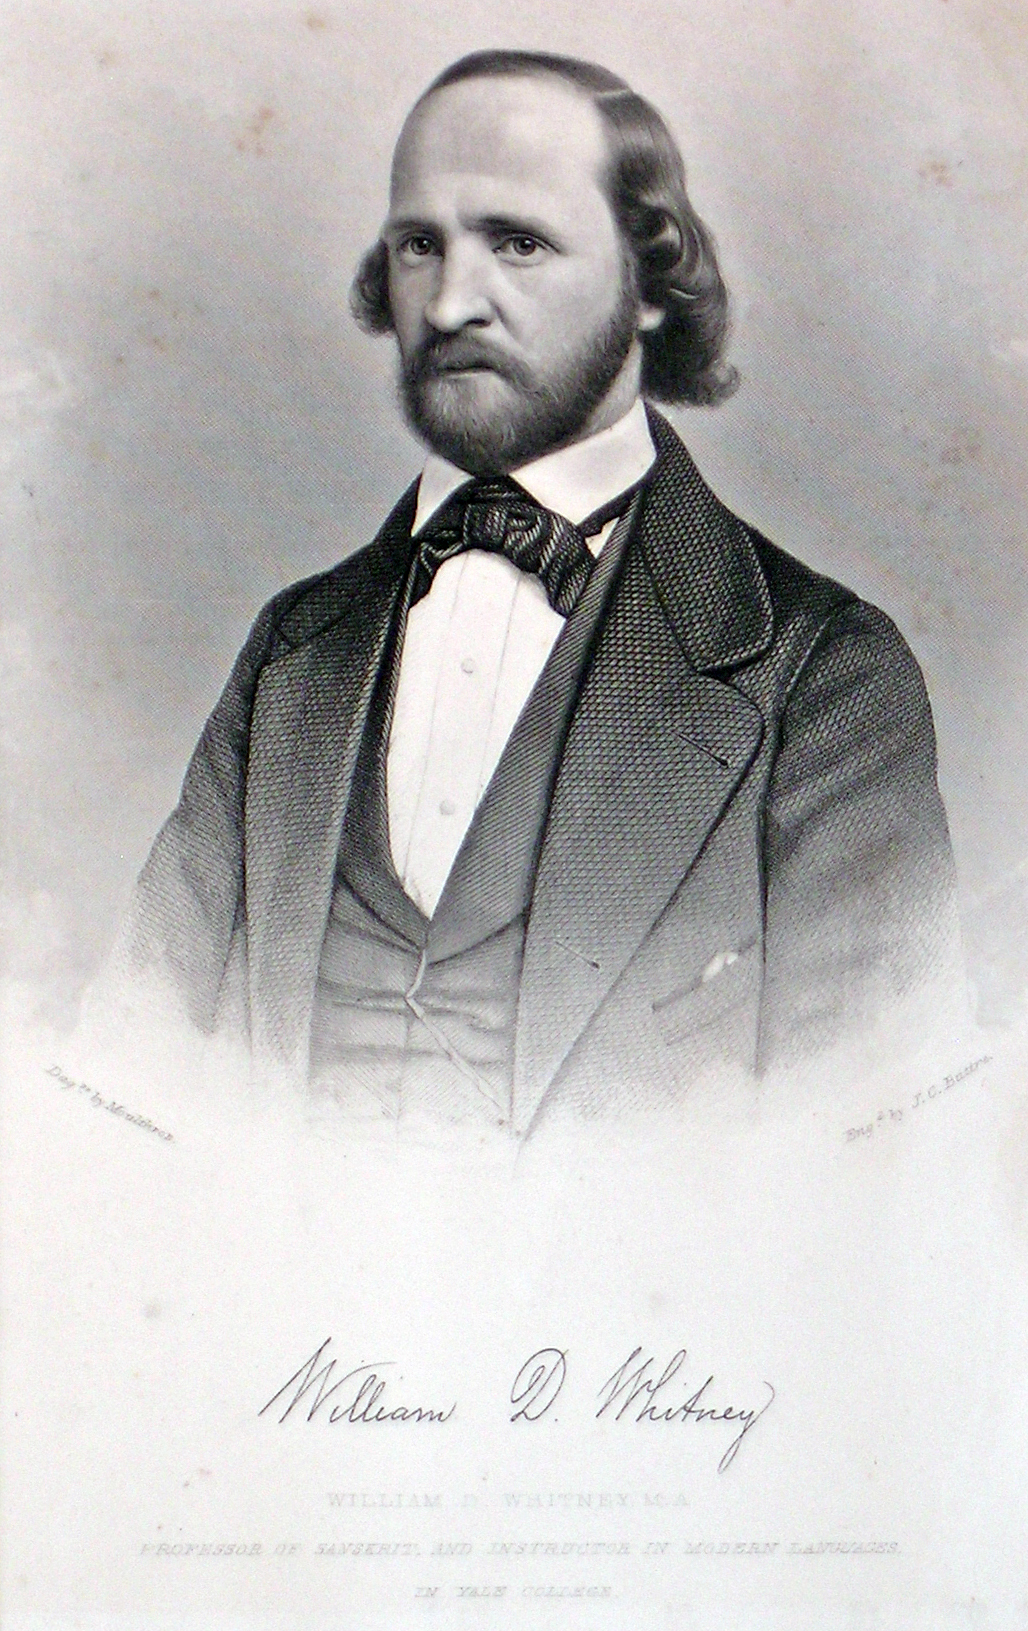
\includegraphics[width=.9\textwidth]{figures/Whitney_1858.jpg}
  \caption{William Dwight Whitney (1858)}
  \label{fig:ch.boas.young_whitney}
\end{wrapfigure}
In 1849, {\Whitney}'s brother brought him a copy of
\posscitet{bopp27:skt} \ili{Sanskrit} grammar from Europe, and this
immediately became a source of fascination to him. He studied \ili{Sanskrit}
at Yale in 1849, and then went to Berlin to continue this study. He
devoted particular attention to the Vedic texts, and prepared what
became the definitive edition of one of these, the Atharva Veda. In
1854 he returned to Yale; the lack of salary for a professor of
\ili{Sanskrit}, however, required him to teach \ili{French} and \ili{German} as well in
order to support his family. In 1870, he had become sufficiently
eminent that Yale was concerned to prevent his moving to Harvard, and
a chair was created for him by \name{Edward}{Salisbury}, his mentor and the
then Professor of {Arabic} and {Sanskrit} Languages and Literature.

Throughout his life, Whitney was active in the scholarly societies
concerned with language (the American Oriental Society, the American
Philological Society, the Modern Language Association, etc.). He
published a number of papers on Indic and \ili{Indo-European} topics as well
as pedagogically motivated works on \ili{French} and \ili{German}. Undoubtedly his
\textsl{\ili{Sanskrit} Grammar} \citep{whitney79:skt.grammar} is his single
best-known work; this model \isi{descriptive study} of the language retains
significant interest for both the Sanskritist and the general linguist
today, and is a major source of information for the details of
{\Whitney}'s view of linguistic structure (see
\citealt{mccawley67:whitney}). At the time, it was well enough
received to establish his credentials as a major figure in
\ili{Indo-European} studies.

In addition to his descriptive and historical linguistic work, {\Whitney}
also published two books on general linguistics: \textsl{Language and
  the Study of Language} \citep{whitney67:language}, and \textsl{The
  Life and Growth of Language} \citep{whitney75:life.and.growth}. Both
of these volumes were known to European scholars: {\DeCourtenay}, {\Saussure}, and {\Fortunatov} among others mention {\Whitney}'s
general linguistic work as sound and interesting, and assigned it to
their students to read. At {\Whitney}'s death in 1894, an international
symposium was organized in his memory to which virtually every
well-known figure in the linguistic world of the time
contributed. Even Saussure wrote extensive notes for an appreciation
of {\Whitney}, though he never completed the article. At the time,
{\Whitney} was probably the one American scholar who was known and
esteemed in world linguistic circles.

\begin{wrapfigure}{r}{.35\textwidth}
  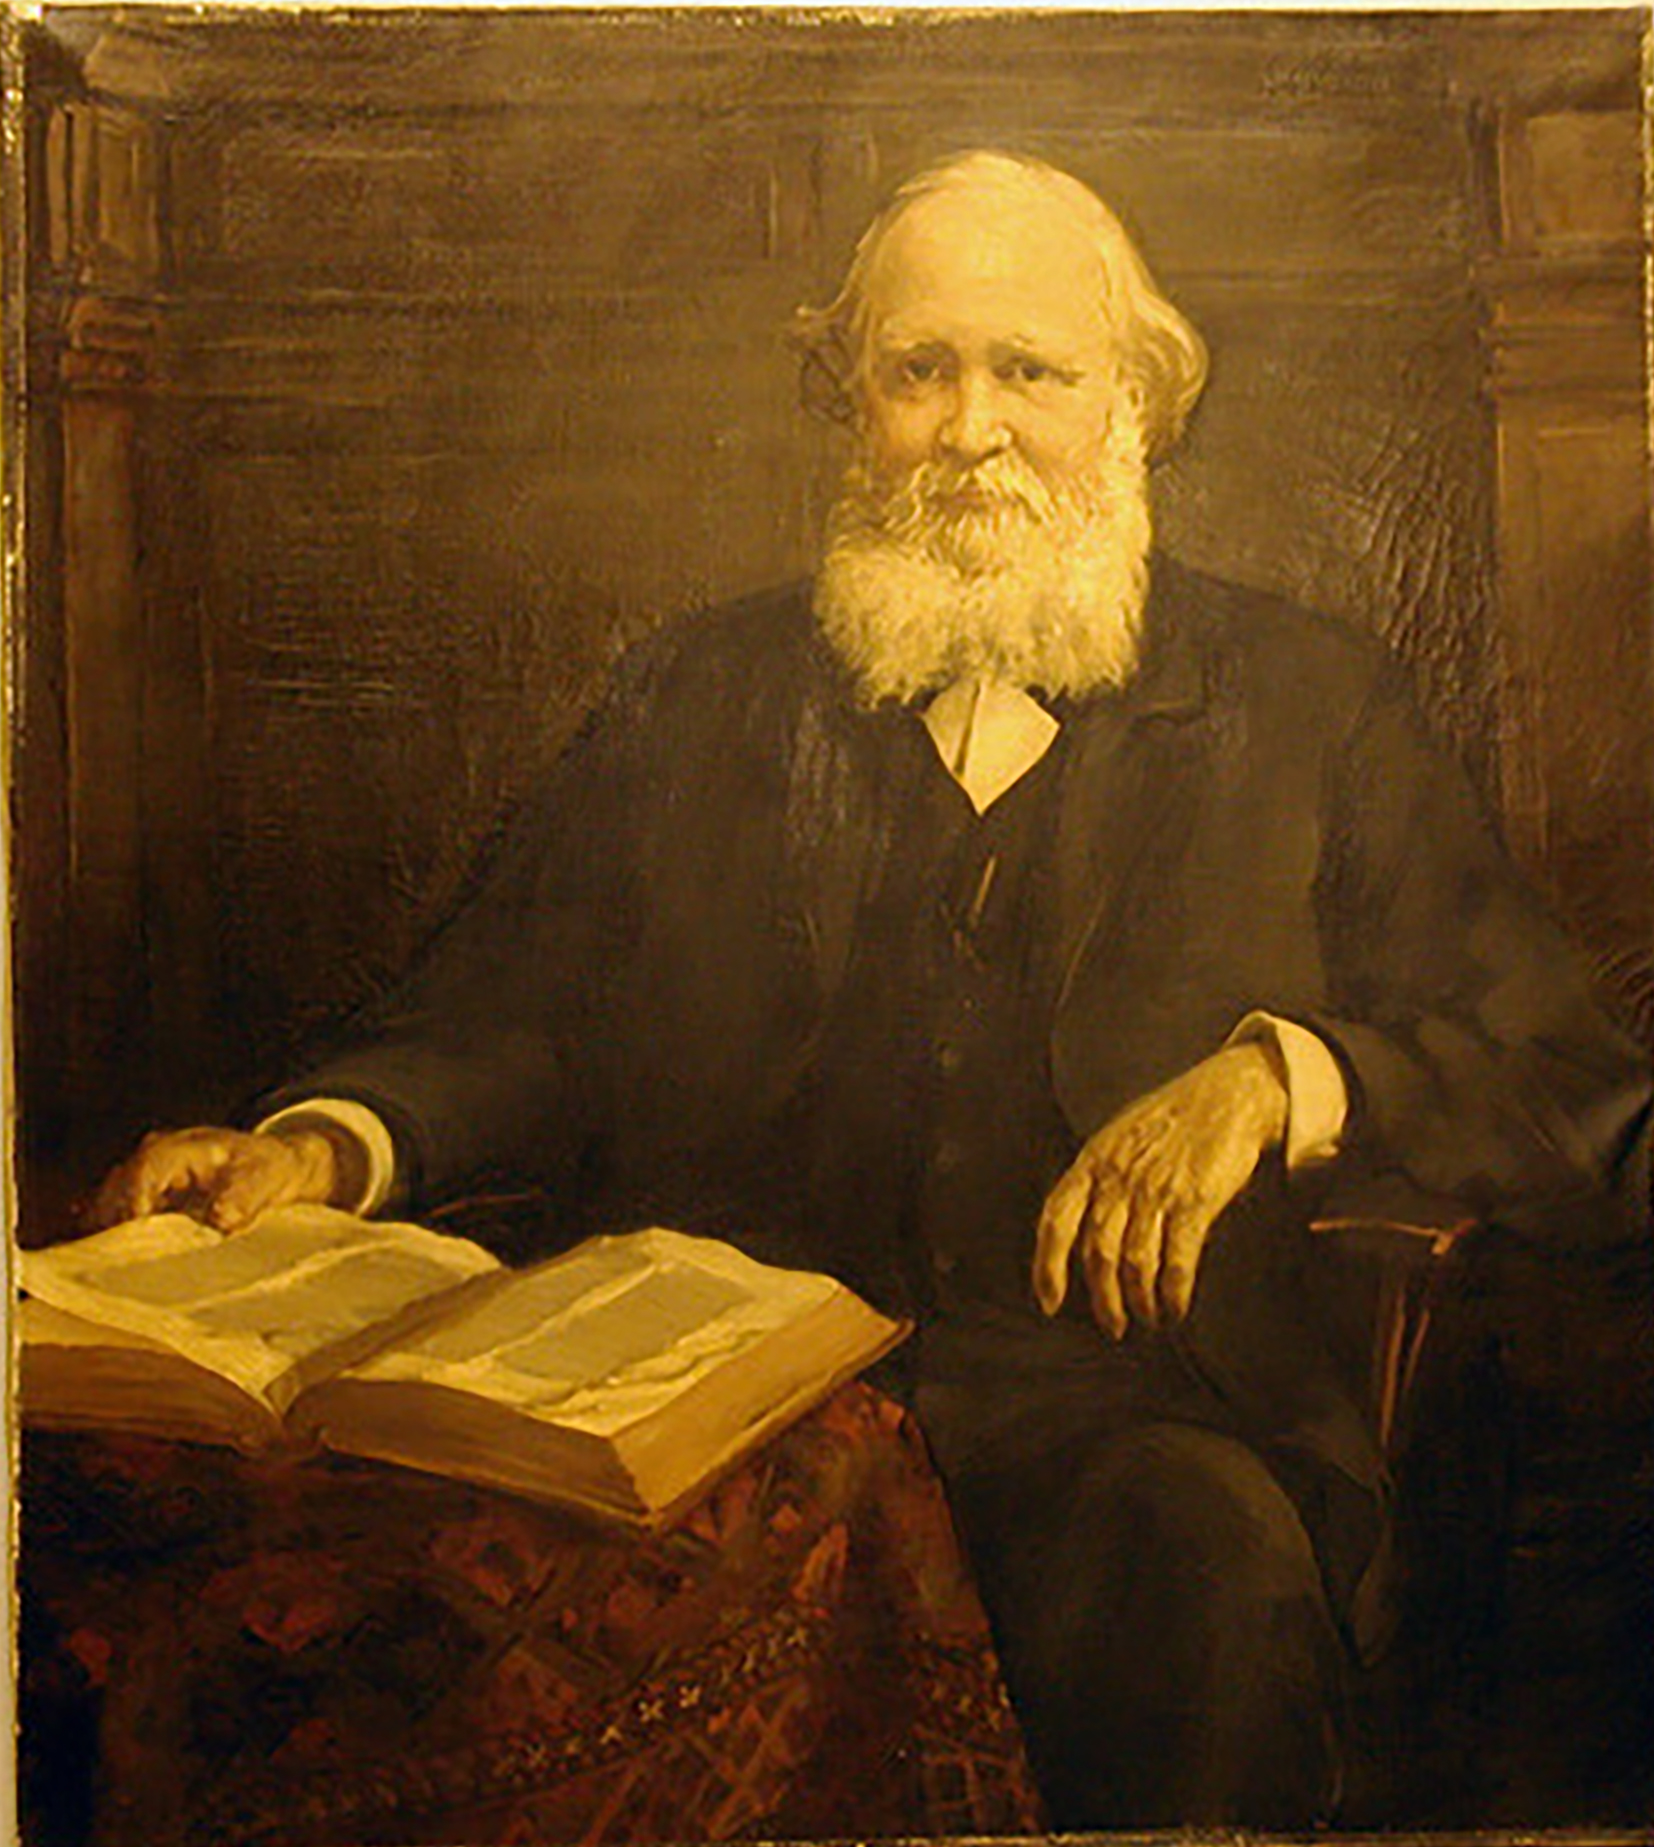
\includegraphics[width=.9\textwidth]{figures/Whitney_painting.jpg}
  \caption{William Dwight Whitney}
  \label{fig:ch.boas.whitney_painting}
\end{wrapfigure}
If we go beyond these biographical details to ask about {\Whitney}'s
impact on the development of linguistics, however, it is difficult to
identify much in the way of innovative propositions concerning the
nature of language that originate with him, or major effects he had on
the field. He was known less for revolutionary or even novel ideas
than for the balance and common sense with which he confronted the
often rather mystical excesses of much other nineteenth-century
thought about language. He was particularly opposed to the views of
Bopp\ia{Bopp, Franz}, {\Schleicher}, and others, who treated language as some sort of
`natural organism' subject to growth, evolution, and decay in an
oversimplified biological way; and he devoted particular energy to
combating the mechanistic views of \name{Max}{Müller}. To these opinions he
opposed an emphasis on the social character of language, with the
effect primarily of countering the prevalent metaphysical speculation
concerning the `organic' nature of language.

{\Whitney}'s main contribution to the field was thus probably in clearing
the air of counterproductive, overly biological or mechanistic views
of language, and in preparing the way for others to pursue more
genuinely linguistic lines of thought. His own work was completely
within the framework of the time, presaging in no important way the
sort of \isi{structuralism} that would soon dominate the field. For example,
an essential preliminary to the `structural' approach to language as
it developed in the twentieth century is an appreciation of the
separation between synchronic and diachronic study, and an abandonment
of the view that \isi{explanation} can be sought only in the history of an
observed state of affairs. There is no evidence at all that {\Whitney}
was ready to make this move; indeed, his background in the study of
geology undoubtedly predisposed him more than most to a historical
view of \isi{explanation}.

Even those who praised him most highly did so in terms other than
those of strict originality: {\Saussure}, for example, observes that
``l'américain {\Whitney}, que je révère, n'a jamais dit un seul mot, sur
les mêmes sujets [i.e., the principles of the study of language] qui
ne fût juste; mais comme tous les autres, il ne songe pas que la
\isi{langue} ait besoin d'une systématique'' (quoted in
\citealt[51]{godel57:sources}). To the practice of linguistics in the
United States at the end of the nineteenth century, {\Whitney} must be
considered to have brought an authoritative presentation of
contemporary European work and a rather common-sensical view of the
nature of language within which more innovative theoretical
understanding was possible (though not yet attained). These were
anything but insignificant contributions; but their importance for the
work of later linguists was preparatory rather than substantive.

\section{Early work on American Indian languages}

Aside from the sort of European-derived historical and comparative
linguistics represented by {\Whitney}, there was another quite distinct
approach to the study of language in North America, which flourished
largely outside of universities. For reasons that were by no means
entirely academic, the languages of the indigenous peoples of the
Americas excited great interest from the time of the first European
contact. Explorers and missionaries, frequently encouraged and
supported by various governments and private sources, accumulated
large amounts of information about these languages dating at least
from the sixteenth century. Though highly uneven in quality, much of
this material preserves its interest today—at a minimum, for the
obvious historical and archival reasons, but occasionally because it
represents work of a high descriptive standard, as in the case of
\name{Roger}{Williams}'s \textsl{A Key into the Language of America}, a
description of the \ili{Algonquian} language \ili{Narragansett} first published in
1643 and available in several modern editions.

Much of this work was conducted by missionaries whose interest in native
languages was driven by the specific, practical purpose of preaching to the
`heathen' and spreading European religion. Similar motivations persist
into the twentieth century and down to the present in the work of such
organizations as the American Bible Society and the Summer Institute
of Linguistics, whose original missionary concerns have led to a great
deal of basic descriptive research on otherwise little-known languages
all over the world, often excellent in quality and commonly our only
available source of information.

Study of the languages of the new world was also stimulated by the
general enlightenment interest in the nature and diversity of
humanity, given the obvious ethnographic fact that the native peoples
of North (and South) America were in most ways very unlike average
Europeans. Already in the early years of exploration of the Americas,
it was recognized that language study was an important component of
\isi{ethnography}: at minimum as a tool for the practical purpose of
communicating with the people under study, and for many investigators
an end in itself.

\begin{wrapfigure}{r}{.4\textwidth}
  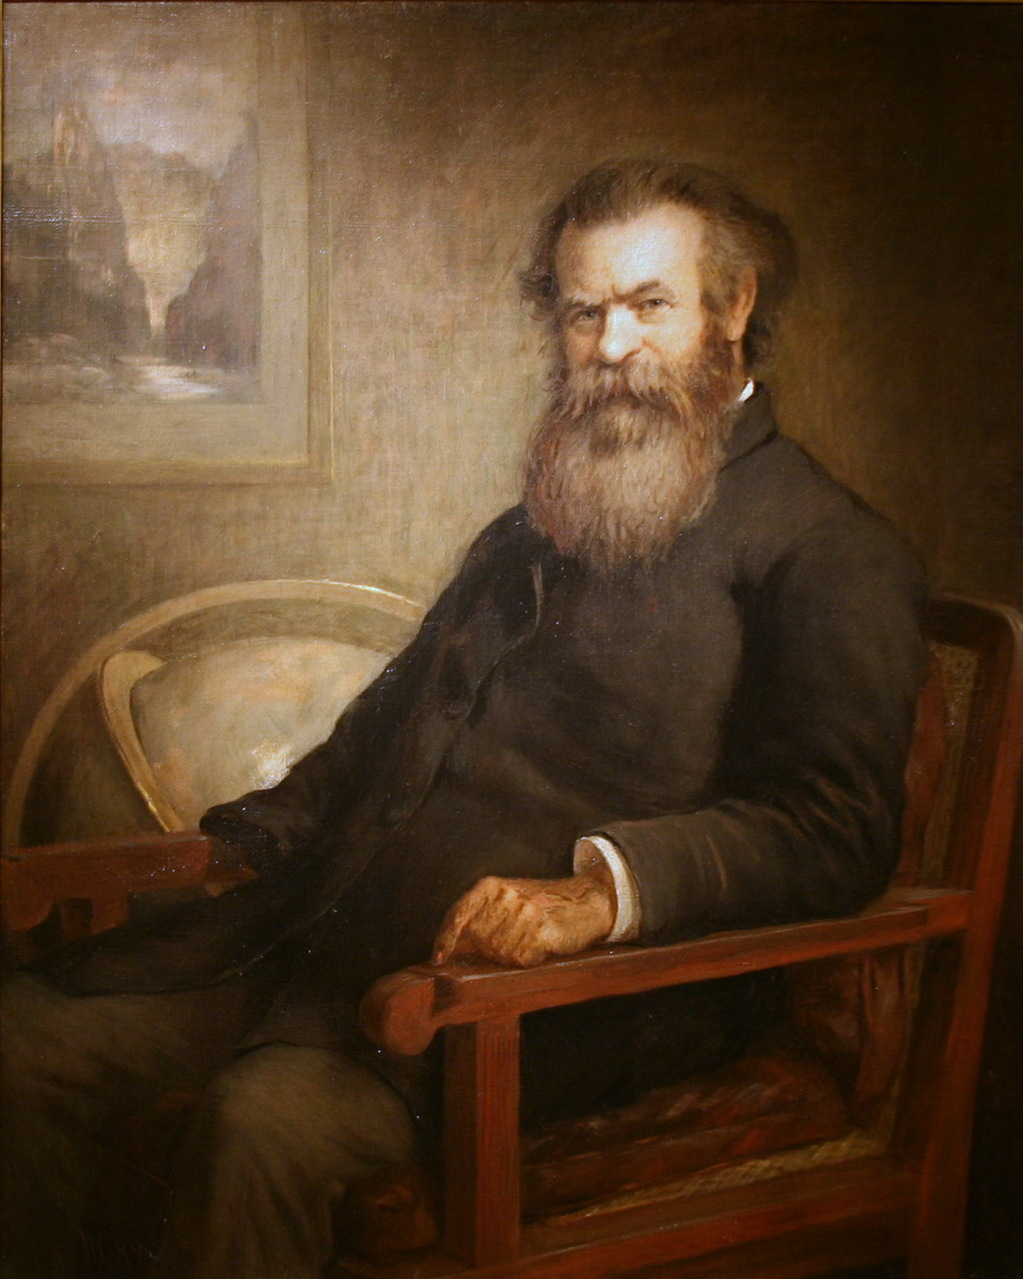
\includegraphics[width=.9\textwidth]{figures/John_Wesley_Powell.jpg}
  \caption{John Wesley Powell}
  \label{fig:ch.boas.powell}
\end{wrapfigure}
In the eighteenth century, much study of Amerindian languages was
institutionalized under the guidance of \name{Peter}{Duponceau} at the
American Philosophical Society (whose previous president, \
name{Thomas}{Jefferson}, had also encouraged the collection of data on North
American languages) and \name{Albert}{Gallatin} of the New York Historical
Society. Both of these men were interested in collecting data from as
many languages as possible, primarily for the purpose of establishing
a classification. Gallatin\ia{Gallatin, Albert}'s work in this area was further developed
and extended in the nineteenth century by \name{John Wesley}{Powell}, in
connection with the U.S. Geological Survey. In 1879, the Bureau of
Ethnology (later called the \isi{Bureau of American Ethnology}) was
established within the Smithsonian Institution, and under the
direction of {\Powell} this became the center of such studies in the
United States.

Most of the research of the \isi{Bureau of American Ethnology} during the
nineteenth century consisted in the collection of word lists from
native languages in a standard form established by {\Powell}, resulting
in classifications that were almost exclusively lexical in
nature. More or less the high point of such research was {\Powell}'s
\textsl{Indian Linguistic Families North of Mexico}, published in
1891. This work, though extensive, produced little information of a
structural or grammatical nature. Such grammatical material as the
Bureau's investigators collected was unrelated to the task of amassing
word lists, and went largely unpublished.

The grammatical accounts (often from missionaries) that did appear
were typically cast in the mold of \ili{Latin} or other traditional grammar:
the sort of description that identifies the nominative, accusative,
dative, genitive, etc., in a language with no overt nominal
inflection, the subjunctive in Chippewa or the ablative absolute in
Siouxan, etc., while paying little or no attention to the major
dissimilarities between these languages and those of Europe. It is of
course potentially interesting to ask how the categories of one
language, such as \ili{Latin}, are expressed in another; but the naiveté of
the work under discussion derives from the assumption that the
grammatical categories of some particular model language (\ili{Latin}) have
a sort of logical primacy that converts such a comparison into an
exhaustive treatment of the language under study.

\section{Franz Boas}

Major changes in the study of Amerindian languages came about as a
result of the influence of \name{Franz}{Boas}, who was largely responsible for
giving such work a more systematic and less anecdotal scientific
basis. Out of this research was to grow a new and quite distinctively
American approach to the study of language in general. `Papa Franz',
as he was referred to by some of his students, is generally regarded
as the father of the authentically scientific study of language in
North America, and this is undoubtedly an accurate picture; but in
fact his influence on the development of the field was rather more
complex than is sometimes assumed.

\begin{wrapfigure}[14]{r}{.3\textwidth}
  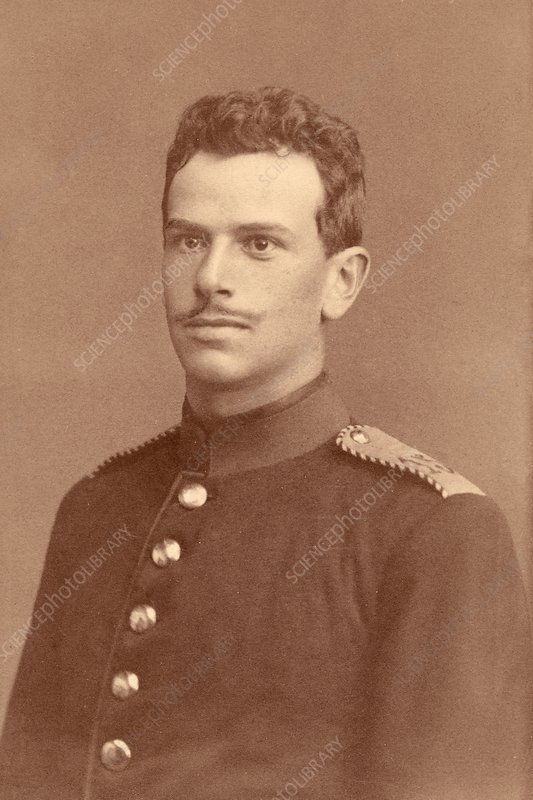
\includegraphics[width=.9\textwidth]{figures/boas_as_student.jpg}
  \caption{Franz Boas as a student [1881]}
  \label{fig:ch.boas.boas_student}
\end{wrapfigure}
Boas\ia{Boas, Franz} was born in Minden, Westphalia in 1858, and studied natural
sciences in Germany. As a student, he was primarily interested in
physics and geography and his training was in those areas rather than
in linguistics or \isi{anthropology}: his PhD from the University of Kiel in
1881 was for a physics project on the optical properties of seawater.
In connection with his geographic studies, though, he became
interested in the possibility of an influence of climate on {culture},
and it was this proposition in part that he was examining when he
first did fieldwork with the Inuit people in 1883, as part of the work
of an expedition to Baffin Island.

Returning to Berlin, he worked at the Royal Ethnological Museum, and
while there, he became interested in the Native Americans of the
Pacific Northwest. After defending a habilitation thesis
\textsl{Baffin Land} in 1886, he left on a three month field trip to
British Columbia, after which he remained in the United States. He was
offered a job as Assistant editor of \textsl{Science}, and was also
appointed as a docent in Anthropology at Clark University, where he
was later made head of a new department.  Over the following years he
became familiar with a number of other peoples of the northwest coast
of North America through his participation in various expeditions
sponsored by {German} and British scientific societies.

Since {\Boas} was completely untaught in the field of linguistics, he was
at first unable to conduct research in this area himself. On his first
field trips he had the services of another investigator, \name{H. J.}{Rink}, a
Dane who had lived among the Inuit of Greenland for a number of years
and who was in fact responsible for nearly all of the linguistic
analysis of Inuktitut material collected. As his interests became more
clearly focused on general ethnographic questions, however, {\Boas}
developed the necessary skills for recording and analyzing the
cultural materials he collected during a decade of work on the
Northwest Coast.

While it is clear that he had a general acquaintance (acquired through
reading rather than formal study) with both the European philological
tradition and American studies of the languages he worked on, it is
also clear that his methods and the view of language they entailed
were essentially worked out by him on his own as a consequence (and
necessity) of the activity of doing fieldwork. Though his first work
was in the tradition of collecting vocabulary lists and examining
genetic relationships on this basis, he had become interested by
around 1890 in deeper problems of the grammatical structures of the
languages under investigation.

In 1892, {\Boas} was engaged to prepare material for the 1893 Columbian
Exposition in Chicago, and travelled north to engage a group of
Kwakwa̱̲ka̱̲ʼwakw (``Kwakiutl''\footnote{``Kwakiutl'' is the
  representation in an early missionary \isi{orthography} of the Kwakw'ala
  word {[kʷagʲuɬ]}, which refers to the particular community of
  Kwakwa̱̲ka̱̲ʼwakw people living at Fort Rupert. Despite the fact that
  this word is clearly an ethnonym (ending in the suffix \emph{-uɬ}),
  while the language itself is Kwakw'ala {[kʷakʷʼala]}, consisting of
  the same root /kʷakʷ-/ followed by the suffix \emph{-k'ala} `to make
  sounds typical of [root]', {\Boas} consistently referred both to the
  entire Kwakwa̱̲ka̱̲ʼwakw population and to their language as
  ``Kwakiutl''.}) people to participate in the Exposition. It was
through this activity that he came in contact with 
\name{George}{Hunt},\footnote{For an extensive treatment of the complex relationship
  between {\Boas} and {\Hunt}, see \citet{wilner15:hunt.and.boas}.} a native
speaker of Kwakw'ala, who would later provide the basis for {\Boas}'
extensive work on that language, and his family
(figure~\ref{fig:ch.boas.hunt_family}). Although ethnically half
Tlingit and half {English}, {\Hunt} had grown up with his parents in Tsax̠is
(Fort Rupert) among the Kwakwa̱̲ka̱̲ʼwakw and was thoroughly familiar with
the language and \isi{culture} of the people--- which, with the aid of his
first wife Lucy ({\HuntL}) and after her death in 1908, his second
wife Francine ({\HuntF}), he documented extensively for {\Boas}.

\begin{wrapfigure}{l}{.45\textwidth}
  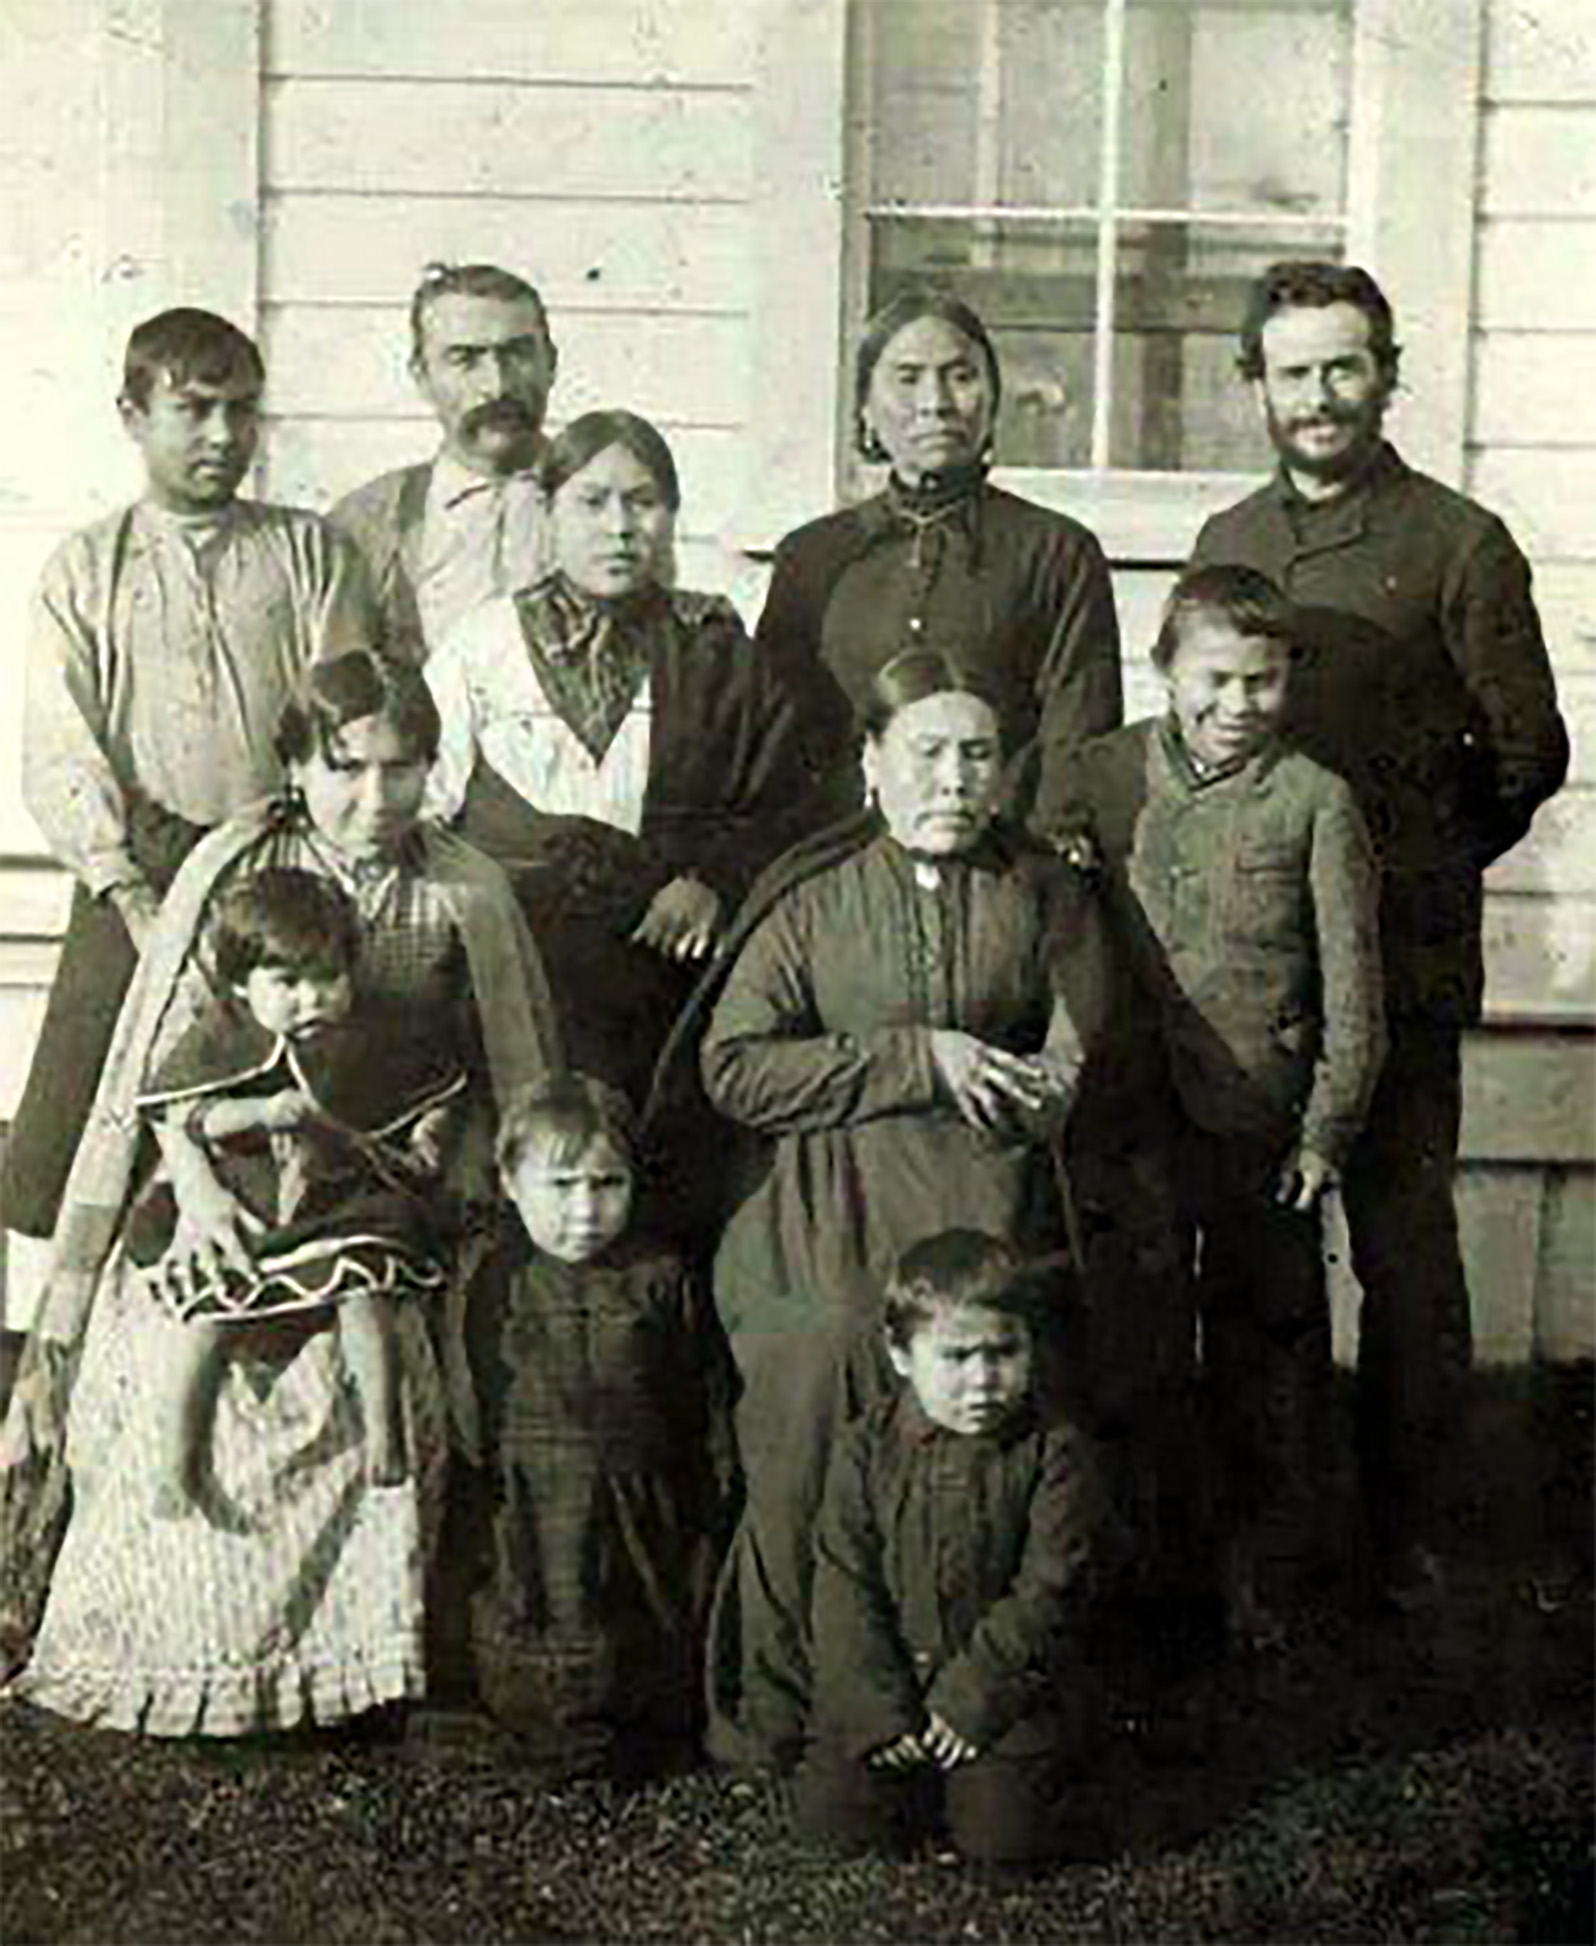
\includegraphics[width=.9\textwidth]{figures/hunt_family_boas.jpg}
  \caption{Boas with George Hunt family 1894 [Back row, left to right:
    Sam Hunt, George Hunt, Mary Ebbetts Hunt (George's mother), Franz
    Boas; standing left to right: Lalaxs'a (wife of David Hunt, not
    pictured), Jonathan Hunt; seated left to right: Emily Hunt
    (holding Marion Hunt), Lucy Hunt; kneeling left to right: Mary
    Hunt, George Hunt Jr.]}
  \label{fig:ch.boas.hunt_family}
\end{wrapfigure}
As {\Boas} did more and more research on the \isi{ethnography} of the northwest
coast of North America, he developed a formal association with museums
in the United States, and with the \isi{Bureau of American Ethnology} under
Powell. He had a position with the Field Museum in Chicago until 1894,
when a \isi{BAE} reorganization resulted in the loss of his job. A year and
a half later he was offered a position in charge of the editorial work
of the \isi{BAE}, but accepted instead an offer to teach at Columbia. He
settled in New York in 1896, and lived there (and taught at Columbia)
until his death in dramatic fashion on December 21, 1942.  While
having dinner in Faculty House at Columbia, he had a heart attack and
fell, limp, into the arms of \name{Claude}{Lévi-Strauss}.

Though {\Boas} was not working for the \isi{BAE}, his influence there grew
considerably as his {competence} as a fieldworker came to be
recognized. At Columbia he made a major effort to train students to do
fieldwork, and within a few years his students represented an
important part of the field research personnel doing work on
linguistic topics under the auspices of the \isi{BAE}. With the development
and final approval in 1903 of the project for the \textsl{Handbook of
  American Indian Languages} (\citealt{boas:handbook_1} and subsequent
volumes, designed to replace {\Powell}'s earlier handbook), {\Boas}
definitely assumed the leading role in the investigation of the native
languages of North America.

{\Boas} exercised in part an influence of a strictly intellectual nature,
since his view of language was passed on to his students at Columbia
and thus came to dominate field research in Amerindian
linguistics. Through his connections with the \isi{BAE} and other agencies,
however, he came to control the major portion of what institutional
support there was for linguistic research in the United States. He had
little respect or tolerance for work he associated with earlier, more
primitive approaches to language, and he saw it as a responsibility to
control research support in such a way as to determine the kind of
work that would be done in the future.

In particular, {\Boas} completely rejected the efforts of missionary
linguists, and as a result such work was not only not supported by
agencies over which he had an influence, but was largely blocked from
publication in channels under his control. His own students and close
associates were the only ones whose work he trusted, and thus he was
somewhat assertive about preventing others from working on languages
on which one of his students was already occupied. When {\Boas} had
`assigned' a given language to one of his students, it became
virtually impossible for anyone else to find any support for studying
it (or even in some cases to penetrate the native community) for an
essentially indefinite length of time—even when the student in
question was not in fact producing any results from the research
intended.

The judgments of the preceding paragraphs on the exclusivity and
proprietary attitude of {\Boas} toward American Indian languages (as well
as the power he exercised in this way) are perhaps
over-generalizations to some degree. In any event, the demonstrated
lack of sophistication of much other work and the limited resources
available for support of linguistic investigation surely made many
apparently harsh decisions necessary if research of importance was to
be supported. The need to make such choices, combined with the extent
(unequaled before or since) to which the power and responsibility
related to them were concentrated in a single person, inevitably led
to the effective exclusion from the field of many whose major failing
was not belonging to the circle of those whose work {\Boas} approved of.

As a result, it seems necessary to identify not only the (massive)
positive aspects of {\Boas}'s contribution to American linguistics, which
we will discuss at length below, but also a darker side of his legacy
to Amerindian studies: an extreme degree of `territoriality' among
Americanists, which persists to the pre\-sent. While there are of course
many notable exceptions, a great many linguists working on these
languages would much rather have a newcomer to the area work on
somebody else's language or family than on their own, and feel that
once a language has been undertaken by a given investigator with the
approval of the scholarly power structure, it is inappropriate for
others to encroach on the same linguistic territory—independent of the
complexity of the language in question or the extent to which research
on it is actually being made available to a larger public. In recent
years, as Native American communities have become more invested in the
intellectual legacy of their languages and increasingly taken control
of their own cultural property, the extent of such influence has
greatly waned, but for much of the twentieth century it was a
significant factor in American linguistics.

For {\Boas}, such apparent protectionism was simply the only way to
ensure that a reasonable scholarly standard replaced what he saw as
the inadequacy and lack of sophistication of the then-existing
descriptive tradition in American linguistics. He was concerned that
the languages of North America be described in sufficient depth to
allow meaningful conclusions about their structure, and also to allow
for adequate interpretation of text material of ethnographic interest.

Indeed, these anthropological (as opposed to purely linguistic)
considerations were generally uppermost in {\Boas}'s mind, and he
stressed the accurate recording of extensive texts (often in the face
of objections to the cost of publishing such material) as a central
activity of the linguistic
fieldworker.\footnote{\citet{silverstein15:boas} discusses the origins
  and importance of {\Boas}' attitude toward the collection and
  preservation of extensive textual material.} It is important to keep
this ethnographic basis of his concern with language in mind in order
to understand some features of his views.

{\Boas} took up linguistic work originally as a necessary tool for the
investigation of \isi{culture}, language being a particularly revealing
aspect of \isi{culture}. Language for him provided a ``window on the mind,''
whose special virtue is the largely unconscious character of the
knowledge it represents. By virtue of this unconscious nature,
language is not subject to the sort of \emph{ex post facto}
rationalization which distorts other expressions of \isi{culture}, and an
understanding of the structure of the language of a people thus
provides a purer approach to their \isi{culture} than the direct study of
other institutions. The collection and study of texts in the native
language was therefore both the only way to penetrate the nature of a
society, and a particularly privileged way to approach the mind of
those who live within the framework established by a given
\isi{culture}. Historical linguistics also had a similar role to play,
insofar as the study of language history furnishes clues to \isi{culture}
history.

{\Boas} quickly discovered in his earliest fieldwork that his initial
notion of an influence of climate on language was thoroughly
misconceived (and he goes to the trouble of refuting any such
connection in the Introduction to the \textsl{Handbook},
\citealt{boas11:introduction}). His interests changed to a concern
with genetic linguistics and the bases for establishing such
relationships among languages. In 1888, and again later, he argued
that Tlingit, Haida, and perhaps Athabaskan were related to one
another—a relationship that rested on no particular vocabulary
comparisons of the usual sort but, rather, on presumed structural
similarities.\footnote{See \citealt{levine79:nadene} for a critical review of
the evidence that led {\Boas}, and later {\Sapir}, to this conclusion}

Based on his experience on the Northwest Coast, however, {\Boas}
gradually came to believe that effects such as borrowing, independent
development of common features, and a general mutual \isi{assimilation} of
structural features within an area were so prevalent as to render
significant historical classification of most North American languages
impossible (or at least of limited interest) ``in the present state of
knowledge.'' He thus became increasingly skeptical of claims of genetic
relationship between languages, and shifted his attention from
historical to synchronic descriptions.

As a partial replacement for the apparent inadequacies of historical
comparison, typological studies based on such accounts might provide a
valid method for comparing languages. Indeed, it has been suggested by
\citet{voegelin52:boas} and \citet{stocking74:boas} that much of the
uniformity in the presentation of various languages in the
\textsl{Handbook of American Indian Languages} is due not so much to a
coherent and uniform theory of language as to the desire to provide a
common expository format that would facilitate such typological
comparison.

\section{Linguistic theory and Boas's \textsl{Handbook}}

The \textsl{Handbook of American Indian Languages} marks a major
turning point in the study of linguistics in America. Originally
conceived as a series of sketches which would replace {\Powell}'s earlier
survey with a presentation of Amerindian language structures in
greater depth, the work came to have a much wider significance than
this. Even disregarding the actual content of the \textsl{Handbook}
sketches, the choices that were made in organizing this first
large-scale effort to describe these languages had lasting
consequences. On the one hand, the selection of authors had the effect
of establishing a relative uniformity with regard to the `linguistic
politics' of the developing field; and, on the other, the
comparatively uniform format and style of presentation of the
\textsl{Handbook} descriptions served as a model for the organization
of grammar which was highly influential in determining the topics
investigated by later workers.

More central, however, was the overt, substantive contribution made by
the \textsl{Handbook} to the formation of American linguists'
views. \posscitet{boas11:introduction} ``Introduction'' argues
persuasively, in concise and highly readable form, for a general
approach to language that stresses the sufficiency and internal
consistency of each individual language without regard to its
adherence to the grammatical or conceptual system of another. {\Boas}'s
point was that each language should be studied in its own terms rather
than examined only through the optic of some other (presumptively
`ideally logical') system; this seems so obvious today as hardly to be
a possible source of major revolution, but it suffices to read a few
eighteenth- and nineteenth-century descriptions of North American (or
other `exotic') languages to convince oneself of the major {change} it
represented.

{\Boas}'s insistence on approaching each language in terms of its
individual features would become, as argued
by \citet{teeter64:triviality}, the basis for the characteristic
position of later American \isi{structuralism} ``that languages could differ
from each other without limit and in unpredictable ways''
\citep[96]{joos57:readings}. Actually, though, there are subtle but
important differences between the view expressed in the Introduction
to the \textsl{Handbook} and the interpretation given it in later
work. {\Boas} did indeed {stress} that languages are not all variants of
the same basic scheme which could be found in nearly pure form in some
one model language; but to say that comparison between languages does
not reveal all of their structure is not to say that they are
incomparable.

The requirement that a new language be approached without a particular
set of preconceptions about its structure did not entail that there is
no universal framework encompassing language structures, or that
differences among languages can be arbitrarily great. Rather, {\Boas}'s
point was that no universally adequate conceptual framework existed at
the time and, more importantly, that no particular language could
furnish in itself an adequate framework for the understanding of all
others. {\Boas}'s views in fact presuppose (and to some extent, argue
for) an underlying system of linguistic \isi{universals} which determine the
range of possible structures of human languages, and which is itself
the proper object of investigation for general linguistics.

In relation to \isi{sound structure}, for example, he discusses the range of
articulatory capacities of the human vocal apparatus. He concludes
that ``the number of sounds that may be produced in this manner is
unlimited'' \citep[15]{boas11:introduction}, which has the consequence
that the set of sounds used by one language does not suffice to
categorize those used by another. Nonetheless, ``each dialect has its
own characteristic phonetic system, in which each sound is nearly
fixed, although subject to slight modifications which are due to
accidents or to the effect of surrounding sounds \ldots\ One of the
most important facts relating to the phonetics of human speech is,
that every single language has a definite and limited group of sounds,
and that the number of those used in any particular dialect is never
excessively large'' \citep[16]{boas11:introduction}.

The thrust of this observation is that, while the number of sound
types available to natural languages may be unlimited, the sorts of
things that are possible as sound systems are not unlimited at
all. Rather, an inventory of possible sounds can be specified in
advance, as a function of human articulatory capacities, and each
language makes its own particular, distinctive, and limited selection
from this antecedently given class of possible sounds. There is a
perfectly good universal theory of the sounds of language to be found
in such a characterization; but such a theory cannot be equated with
the particular sound inventory of any specific language or group of
languages.

A similar observation is made with respect to the range of ``groups of
ideas that find expression in fixed phonetic
groups'' \citep[24]{boas11:introduction}. Again there is an inventory of
possible ideas which can be so expressed; this inventory, like that of
possible sounds, is not limited to some finite number, but this does
not mean that no theory of the range of possible ideas could
exist. There exists no obvious and direct basis for a theory of this
sort, such as is provided for a theory of \isi{sound structure} by the facts
of the articulatory capacities of man, but this hardly precludes the
claim that linguistically expressed ideas are taken from some
universally available set.

Of course, as in the case of sound systems, each language makes its
own selection from this set, and the selection made by one language is
quite independent of that made by another. The finiteness of this
selection is argued to follow as a theorem from the finiteness of the
expressive range of the phonetic system, with the further result that
``since the total range of personal experience which language serves to
express is infinitely varied, and its whole scope must be expressed by
a limited number of phonetic groups, it is obvious that an extended
classification of experience must underlie all articulate speech''
\citep[24]{boas11:introduction}. While we will never understand the
grammatical classification imposed by a given language if we limit
ourselves to the categories available in some other language, this
does not at all entail that there could be no general understanding of
the range of ideas systematically expressible in language.

The system of grammatical categories in any particular language is not
simply an inventory of ideas which that language \emph{can} express in
determinate ways, but also a range of concepts which \emph{must} be
expressed in that language. Since these systems differ from language
to language, important differences between systems may rest less on
what is possible than on what is obligatory. In \ili{English}, for example,
noun phrases necessarily indicate the number (singular or plural) of
their referent, and the category of definiteness; verbs are
necessarily marked to indicate tense. By comparison, \ili{Kwakw'ala} noun
phrases contain no necessary mark of the distinction between singular
and plural, or of definiteness; and \ili{Kwakw'ala} verbs have no necessary
indication of tense. On the other hand, \ili{Kwakw'ala} noun phrases must
indicate the deictic relation between the speaker and the referent,
and \ili{Kwakw'ala} verbs must indicate whether the action referred to was
actually witnessed, learned about by hearsay, or took place in a
dream.

The point is not that the categories of one language cannot be
expressed in the other: \ili{Kwakw'ala} speakers have perfectly good ways of
indicating number, tense, etc., when these categories are essential to
an understanding of the situation described, just as \ili{English} speakers
can indicate how an object is located with respect to the speaker, or
the fact that something described took place in a dream. The
fundamental influence of a particular grammatical system lies not in a
limitation on expressive power but in differences in the range of
categories with respect to which a speaker is required to make a commitment
(like it or not) in any utterance in the language in question.

A given language is characterized by its own selection from the range
of possible sound systems, then, and also by its selection from the
range of possible ideas which may (or must) be expressed as
grammatical categories. Furthermore, ``in the languages of the world,
the number of processes which are utilized to express the relations of
terms is limited \ldots\ The only methods that are available for
expressing the relations between definite phonetic groups are their
composition in definite order, which may be combined with a mutual
phonetic influence of the component elements upon one another, and
inner modification of the phonetic groups themselves''
\citep[27]{boas11:introduction}. The range of morphological devices
available for systematic exploitation, then, is subject to very strict
substantive limitation—much narrower, in fact, than the limitations on
sound systems and on semantic/grammatical systems.

This picture, then, does not at all entail a rejection of the notion
of \isi{universals} of linguistic structure, though that was the
interpretation often given to {\Boas}'s views (at least rhetorically) by
his successors in seeking to distance themselves from what they saw as
the excesses of traditional approaches to language. In part, no doubt,
there was a component of simple chauvinism in this: an attempt to
identify a distinctively `American' linguistics. By founding their
methods on a radical and eye-catching exaggeration of a fundamentally
common sense principle, later investigators sought to \isi{stress} the
special and independent character of linguistics in America. In
essence, however, {\Boas}'s insight (while fundamental) was not quite so
dramatic as advertised, and consisted essentially of the observation
that an adequate universal theory of language could not be founded
exclusively on the facts of a single `model' language or group of
languages.

\section{Boas's views of phonology}

When we seek to understand {\Boas}'s own picture of \isi{sound structure}, it
is necessary to rely on indirect evidence to supplement his limited
explicit treatments of the subject. The discussions of phonetics
(broadly construed to include everything from the details of
\isi{articulation} through comparatively abstract morphophonemic
alternations) in the Introduction to \textsl{The Handbook of American
  Indian Languages} and in individual descriptive studies of
particular languages are not really focused on a program of developing
a general \emph{theory} of such structure; what they seek to establish
is an adequate and consistent practice. Given {\Boas}'s central interest
in \isi{ethnography} rather than in the study of language \emph{per se}, it
is natural that morphology and syntax (the formal correlates of the
domain of \isi{meaning}) occupied much more of his attention.

As stressed by \citet{mackert94:boas} and
\citet{silverstein21:boas.sapir.bloomfield}, {\Boas} was well acquainted
with nineteenth century theories of \isi{acoustics}, \isi{articulation} and
perception as these applied to speech, and these provided the basis
for his views on specific issues. Apart from an interest in providing
a comprehensive general system for transcribing and recording the
sounds of unfamiliar languages such as those of Native America that
would replace earlier unstisfactory systems such as that associated
with {\Powell}'s work\footnote{This was implemented as
  \citealt{boas.etal16:transcription}, a project originated by {\Sapir}.
  The history of the committee's work that produced this report is
  detailed by \citealt{silverstein91:rvw.darnell}.}, and to avoid some
common misconceptions about the phonetic resources of such languages,
his theoretical interest in this area was minimal.

It is, of course, worth making the effort to reconstruct as complete a
picture as possible of {\Boas}'s views. In part this enterprise is
interesting in its own right: the conception of linguistic structure
held by anyone with {\Boas}'s enormous experience of unusual languages
could hardly fail to be worthy of attention. But for historical
purposes, it is especially important to know what {\Boas} thought about
the organization of sound systems in natural languages. An obvious
reason for this is that his views were communicated (whether
explicitly or implicitly) to his students, and thus constituted a
significant influence on their work.

Somewhat less directly, we can note that his notion of \isi{sound structure}
was formed, based on his earlier acquaintance with then-current
theories of \isi{acoustics}, articulatory physiology and psychoacoustics, in
the context of practical fieldwork and informal reading (rather than
explicit instruction) of the linguistic literature of the time, such
as the work of \name{Hermann}{Paul}, \name{Eduard}{Sievers} and other lights of the
Neogrammarian movement. Taken together, these factors lead to the
conclusion that the `theory' of phonology which we may attribute to
him actually represents a sort of consensus about the way in which
languages are organized, prior to the crystallization of more
`theoretical' American linguistic views later in the century. Both
historically and logically, then, {\Boas}'s position represents the
starting point from which later theorizing about phonology in America
would proceed.

If {\Boas} was primarily interested in studying the conceptual
organization of language for ethnographic purposes, he still felt that
an essential preliminary to such study must be the phonetic recording
of texts (and of individual linguistic forms). This first step of
representing accurately the material the linguist collects, then, is
of fundamental importance for the analysis of a language's
structure. Without a method of recording textual material with
sufficient accuracy to allow its faithful reproduction, the linguistic
(or ethnographic) fieldworker is not in a position to confirm any
conclusions that may be drawn from an analysis. This concern for
phonetic accuracy is absolutely essential to {\Boas}'s projects, and
overrides all other considerations in determining the proper way to
represent linguistic material. An understanding of this point is the
key to a number of aspects of {\Boas}'s views.

For example, it is quite clear that the question of whether or not two
sounds are in \isi{contrast} within a given language plays little or no role
for him in determining whether or not they should be recorded with
distinct symbols. Insofar as two sounds are consistently
distinguishable phonetically, it is necessary to reproduce this
distinction in a faithful rendition of texts in which they occur; and
thus the difference should be recorded where it appears, regardless of
whether the analysis seems to indicate that it is a predictable
one. This interpretation is overwhelmingly supported by the evidence
of {\Boas}'s practice in recording and presenting phonetic systems for
descriptive purposes. The inventories of segments which are enumerated
in his various grammars include large numbers of non-contrastive
elements which are quite systematically distinguished in texts and in
example forms.

A good instance of this practice is provided by {\Boas}'s treatment of
the vowel system of Kwakw'ala, the language to which he devoted more
of his attention than any other. In his posthumously published grammar
\citep{boas47:kwakiutl} he regularly distinguishes some seventeen
separate vowels. These distinctions are marked both in the forms cited
in the grammar and in the vast amount of textual material he published
during nearly fifty years of work on the language (mostly, it must be
said, on the basis of material collected and recorded by George
{\Hunt}). Of these, however, at most seven (and more likely six) vowels
are actually in \isi{contrast} with one another. This difference does not in
the least represent a failure on {\Boas}'s part to notice the
\isi{regularities} of distribution in the language: as
\citet{swadesh48:rvw.boas} points out in a review, the
`phonemicization' of the vowel system is quite clear from his
description, and he states plainly the predictabilities that there are
among the vowels; nonetheless, he goes right on writing all of the
predictable variants with distinct symbols.

The question of whether a difference between two sounds is predictable
(or, on the other hand, contrastive) was thus not a matter of
indifference to {\Boas}: if a description were to provide an accurate and
comprehensive analysis, it must state such \isi{regularities} as
characterize the language in question, including predictabilities in
the distribution of phonetic segments. Still, the fact that such
\isi{regularities} form part of the descriptive analysis does not for {\Boas}
entail the conclusion that they determine the nature of a
linguistically significant representation. Stating the relevant rules
as part of the grammar is quite sufficient; if the linguist proceeds
from there to reduce certain predictably distributed segments to a
uniform representation, nothing of significance is gained to
compensate for the resulting potential loss in immediacy and phonetic
accuracy of the \isi{transcription}. {\Boas}'s practice thus corresponds quite
closely (insofar as it is appropriate to interpret it as a theory) to
the `\isi{fully specified surface variant}' view of phonological structure
described above in chapter~\ref{ch.saussure_life}.

\begin{wrapfigure}{l}{.4\textwidth}
  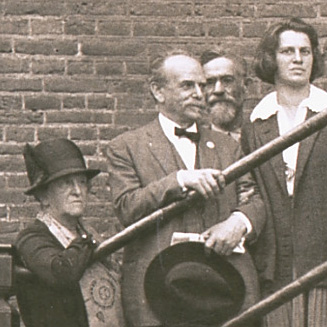
\includegraphics[width=.9\textwidth]{figures/boas_1924.jpg}
  \caption{Franz Boas with his wife and daughter at the 21st
    International Congress of Americanists, The Hague, 1924}
  \label{fig:ch.boas.boas_1924}
\end{wrapfigure}
In the 1920s and 1930s, the notion of a `phonemic' representation was
being articulated, and hailed as a major insight into the nature of
human language. {\Boas} certainly did not disappear personally from the
American linguistic scene during this period; after the publication of
the \textsl{Handbook} and the grammars associated with it, he played a
prominent and forceful role in the development of the field in the
years between the two world wars. There is no reason to doubt his
familiarity with `phonemic' views, but he remained at least
unreceptive (if not outright hostile) to the replacement of phonetic
by phonemic transcriptions as \isi{phonemic theory} gradually took
prominence as the cornerstone of a `scientific' approach to language.

As noted by the last of his students during this period
Amelia Susman {\Schultz}, he was willing to acknowledge the
potential interest of phonemics; after all, the basic insight of all
phonemic views is simply the proposition that a \isi{linguistic description}
must express the fact that some phonetic differences can correspond to
differences of linguistic signs, while others cannot. He did not,
however, encourage his students to make use of phonemic
\isi{representations}, claiming ``that the difference between phonemic and
phonetic writing is only a practical one. I prefer phonetic writing
which does not prejudge the phonemic interpretation. The latter is
given in the phonetic rules which may be verified from the phonetic
writing while they cannot be verified from the phonemic writing. The
more complex the phonetic changes controlled by purely mechanical
conditions the more difficult it is to read phonemic writing'' (from a
letter of 3 August, 1939, cited by
\citealt[56]{schultz77:boas.phonemics}).

Indeed, {\Boas} even rejected a more or less phonemic representation in
cases where it clearly corresponded to the intuition of a native
speaker. A striking instance of this is provided by his treatment of
textual material in Kwakw'ala, which \name{George}{Hunt}, as a native speaker
of the language, had learned from {\Boas} to write. During many years
when {\Boas} was not himself in the field, he employed {\Hunt} to collect
texts for him. In fact, the bulk of {\Boas}'s published Kwakw'ala texts
were written down directly by {\Hunt}, with a great deal of the
information recorded provided by {\Hunt}'s first wife Lucy ({\HuntL})
and his second wife Francine ({\HuntF}). {\Boas} would then go through
them and make certain editorial emendations before sending them for
publication. Among these changes were some more or less systematic
ways in which {\Boas} corrected ``the defect[s] of [{\Hunt}'s] writing'' (as
discussed in \citealt[xi. ff.]{boas30:religion}), in effect so as to make it more
phonetically accurate by restoring non-contrastive differences
eliminated by {\Hunt}.

\begin{wrapfigure}{r}{.5\textwidth}
  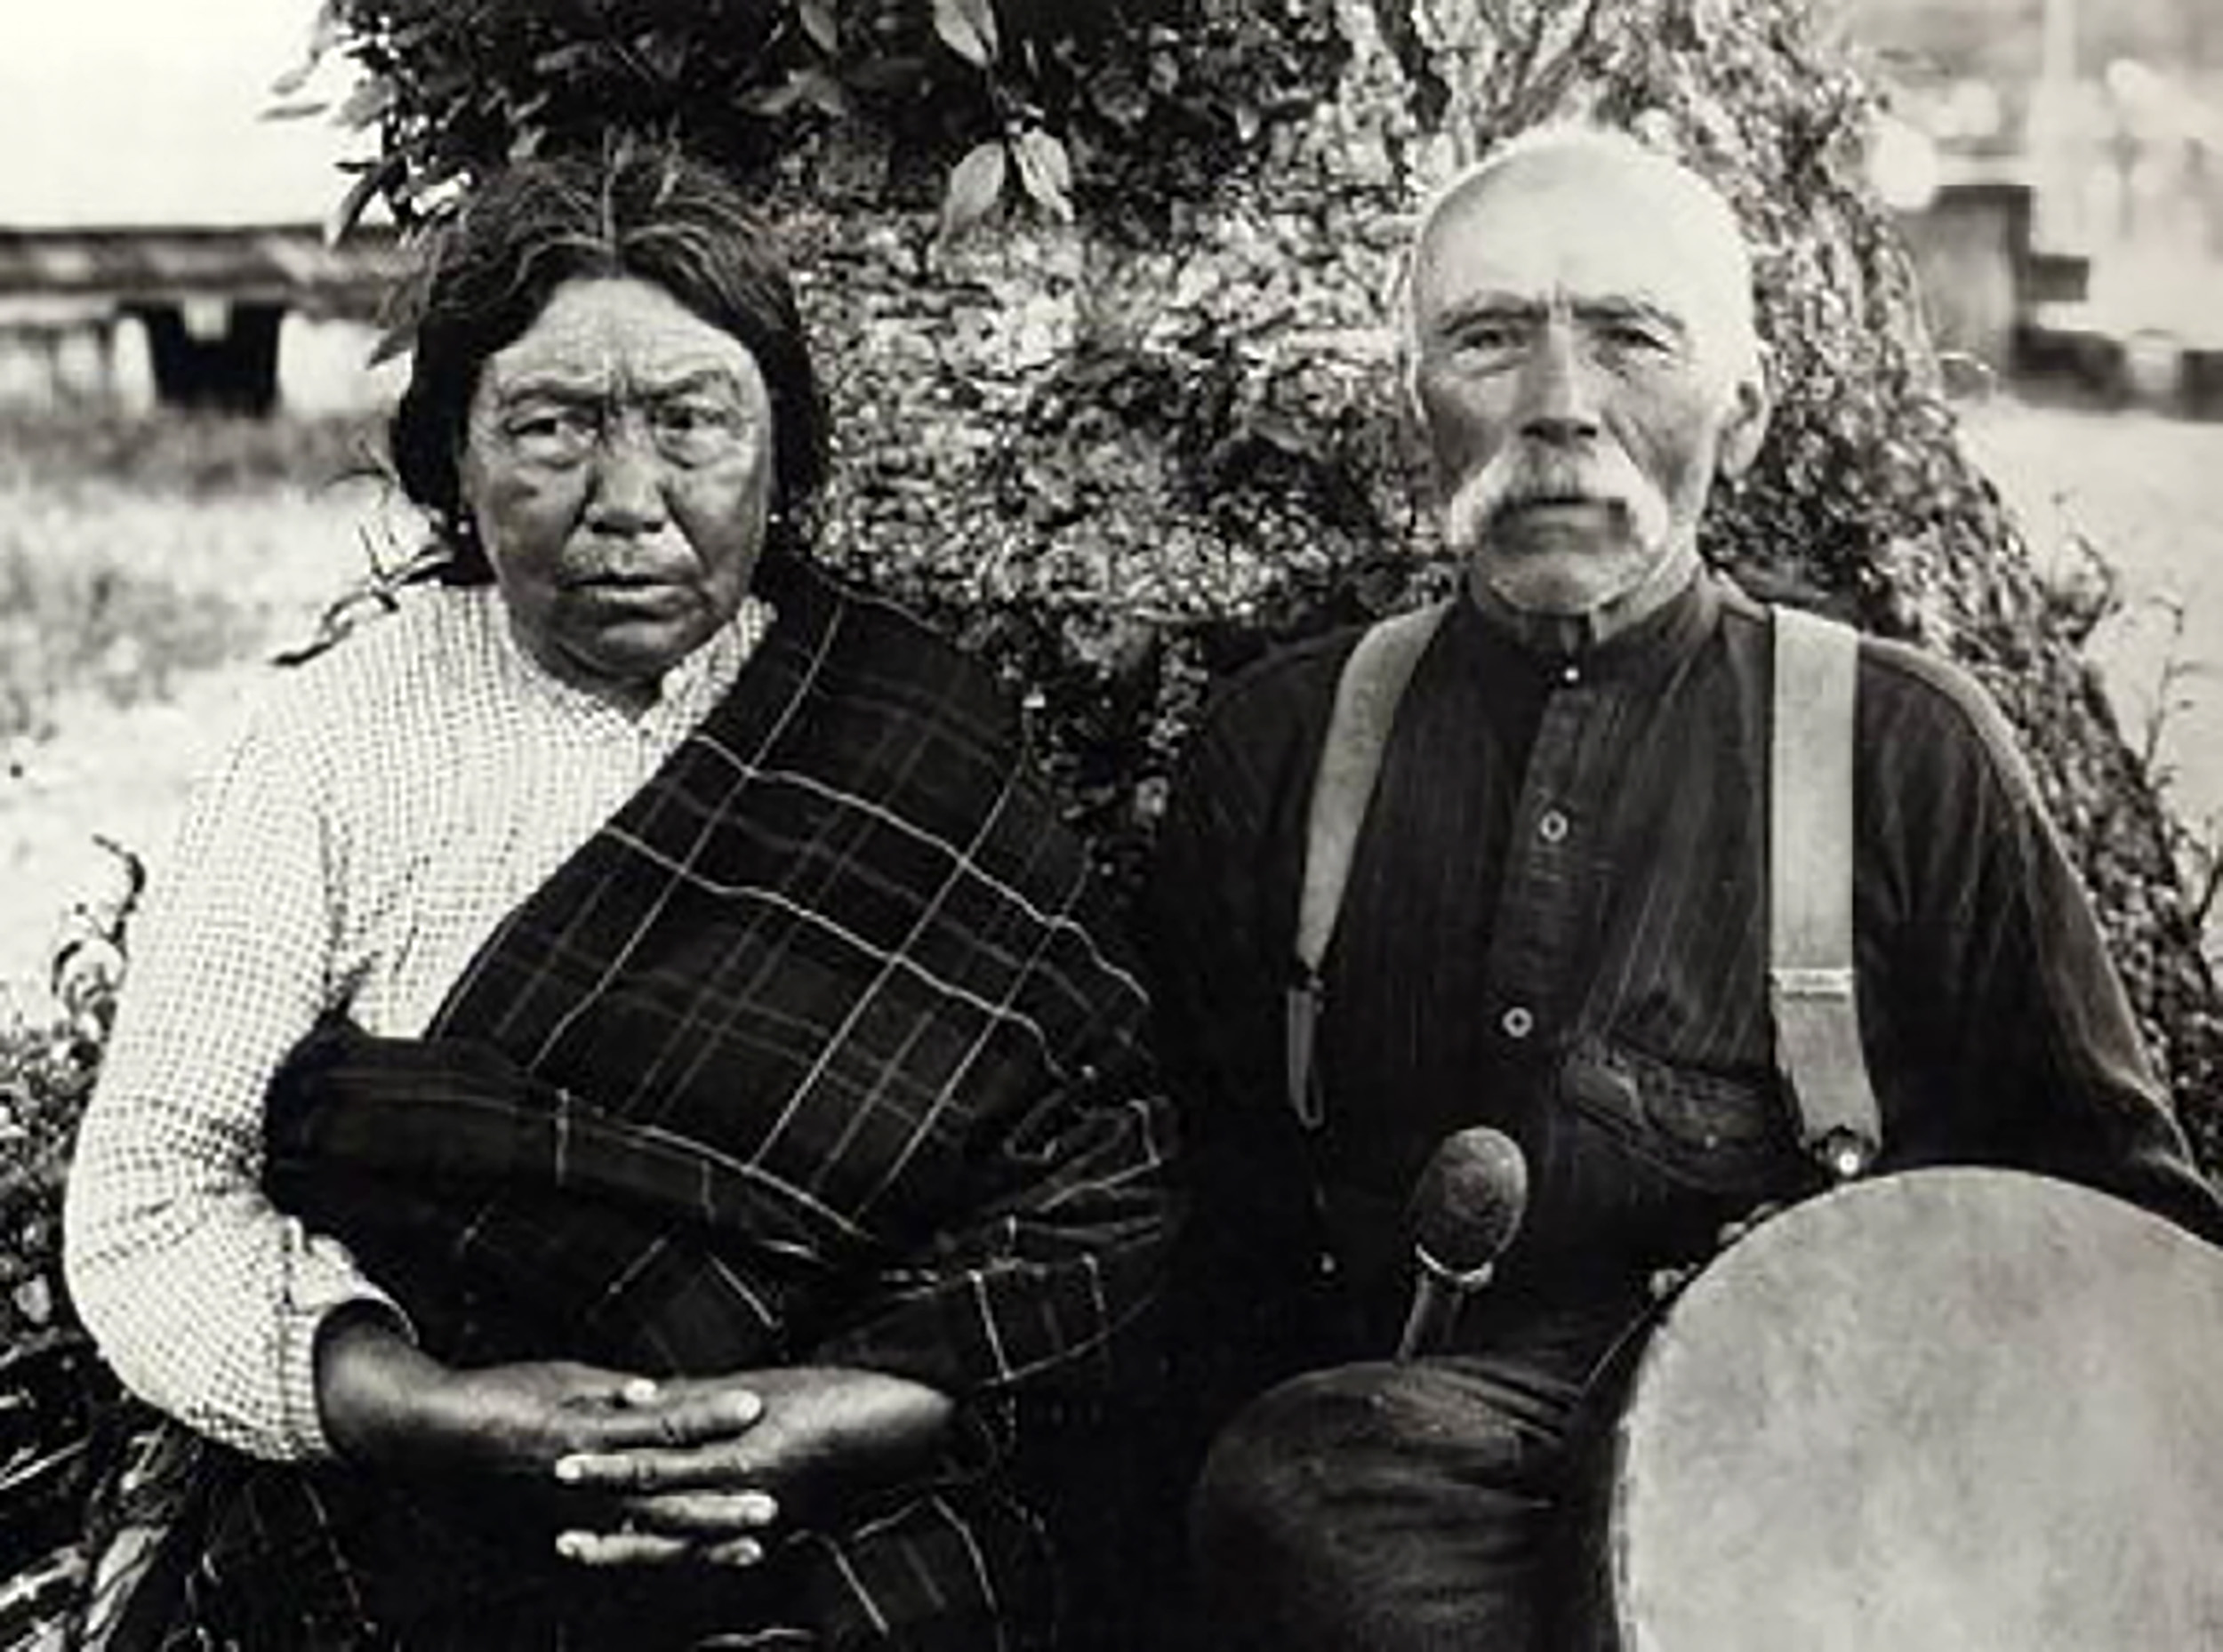
\includegraphics[width=.9\textwidth]{figures/George_Hunt_Tsukwani.jpg}
  \caption{George Hunt and Tsukwani (Tsax̠is, 1930)
  }
  \label{fig:ch.boas.hunt_tsukwani}
\end{wrapfigure}
An important {change} is introduced by {\Boas} in the treatment of the
variants of /ə/. He notes explicitly that this appears as the vowel he
writes <î> when following palatals, as <ŭ> following labialized
\isi{consonants}, and as <ă> after \isi{laryngeals} and uvulars. {\Hunt} (usually)
wrote all of these in the same way: as <{\footnotesize E}> (=[ə]). He
also wrote phonetic [ŭ] after nonlabialized \isi{consonants} as
<w{\footnotesize E}>)—expressing the fact that this sound is a
contextually conditioned variant of [ə]. {\Boas}, however, went through
all of {\Hunt}'s material and `corrected' these interpretations by
restoring the phonetic variants. In \textsl{The Religion of the
  Kwakiutl Indians} \citep[xiv--xviii]{boas30:religion} he presents a
sample text in both {\Hunt}'s and his own, emended, form. Every case of
{\Hunt}'s <{\footnotesize E}> after the appropriate \isi{consonants} has been
replaced by <î>, <ŭ>, or <ă>; and <w{\footnotesize E}> has been
rewritten as <ŭ>. It is obvious here that phonetic literalness not
only dominates the linguist's analysis, but even overrules the native
speaker's intuitions in determining the proper way to represent the
\isi{sound structure} of utterances.

In order to achieve the necessary degree of phonetic accuracy in
recording a strange language, {\Boas} insisted that the investigator must
first of all be free of those predispositions about linguistic sounds
that derive from his own native language and those similar to
it. Given the phonetic capacities of the human vocal apparatus, the
number of actual different sounds that can be produced (and perceived)
is infinite. As noted above, {\Boas} pictured each language as making its
own idiosyncratic selection from among these, a selection which is in
principle completely independent of the selection made by any other
language, and which need not overlap with the sounds used in some such
other language. As a result, the unfamiliar sounds which an
investigator encounters in, for example, Tlingit must be regarded in
their own right, and not as imperfect attempts to produce sounds
familiar from \ili{English}, \ili{French}, \ili{German}, etc.

This might well seem so obvious as not even to bear stating, but in
fact {\Boas} was combating an actual and even pervasive impression in the
literature of his time. Missionaries and other early fieldworkers had
observed that when working on a strange language they often
encountered sound types which presented them with real difficulties
for consistent recording. For instance, in \ili{Pawnee} a sound type was
found which sounded sometimes like [d], sometimes [n], sometimes [l]
or [r]. It had been claimed on the basis of such experiences that
`primitive languages' were in part characterized by such a phenomenon:
they were asserted to contain so-called \emph{alternating sounds}, whose
essence was that they were not articulatorily well defined but mixed
or fluctuating in character.

In an early paper (one of his few explicit discussions of phonological
issues), \citet{boas89:alternating} attacked this notion, claiming
that it was completely illusory. The so-called ``alternating sounds''
are not, he urged, fundamentally different in their degree of
articulatory constancy from those found in familiar languages, but
simply \emph{different} from those with which the investigator is
familiar. In attempting to perceive them in terms of sounds from his
own native language, the fact that they are not fully identical with
any of these leads to an unclear and vacillating perception; but this
is a fact about perception and not about the sound itself.

{\Boas} saw the process by which the ear interprets a sound as mediated
by the apperception of the incoming acoustic signal, grouping it with
one or another of a set of antecedent sound types grounded in the
hearer's prior linguistic experience.\footnote{Further explication of the
assumptions of this model and its historical origins is provided by
\citet{mackert94:boas}.} To the extent a particular
signal does not correspond closely to any of these types, it may be
apperceived sometimes as one, sometimes as another.  A hearer
operating in this way, whose perceptual system is founded on the
sounds of some particular language (perhaps supplemented by exposure
to a few others) will inevitably be ill equipped to respond to sounds
that fall outside the predisposed inventory; but that fact results
from the effects on perception of learning a particular language and
not from any fundamental difference in character between the sounds
of, for example, \ili{German} and \ili{Pawnee}. 

{\Boas} argues for this conclusion from two sorts of fact. On one hand,
sounds of the same language can be shown to be recorded in different
ways by investigators whose own language backgrounds differ. He
suggests that in some cases, it is even possible to determine the
native language of the linguist by looking at the way unfamiliar sound
types are transcribed. On the other hand, the exact same phenomenon is
experienced by speakers of American Indian languages when confronted
with sounds of \ili{English}, \ili{German}, \ili{French}, etc., which are unfamiliar to
them on the basis of their own languages. To a speaker of Tlingit, for
instance, certain sounds (or sound groups) in \ili{English} appear as
`alternating sounds', since their nonoccurrence in Tlingit leads to a
vacillating and inconsistent perception of them (at least at first—but
it is exactly first impressions that matter here, since the sort of
fieldwork on which the `alternating sounds' doctrine was based was
largely a matter of rather superficial exposure for the purposes of
collecting word lists). These two lines of argument converge on the
same conclusion: that the phenomenon of `alternating sounds' is a fact
about the way the ear interprets incoming acoustic material, and not a
characteristic of certain (`primitive') languages.

\section{Representations and rules in Boas's descriptions}

{\Boas}'s position on the question of `alternating sounds' implies that
particular languages classify phonetic segments in such a way that any
sound which fails to \isi{contrast} with a given unit is treated as in some
sense equivalent to it. At least, this is one way of approaching the
phenomenon: if an unfamiliar sound in \ili{Pawnee} does not occur in
\ili{English}, it obviously does not \isi{contrast} with such \ili{English} sounds as
[n], [d], [r], and [l], and so could be assigned to the same category
as any of these, indifferently. We might interpret this as at least a
precursor of later `phonemic' theories, which have in common the
assignment to the same category of sounds that do not \isi{contrast} with
one another.

Actually, however, just the opposite is true, and {\Boas}'s position
represents a consistent view that phonetic substance in its most
literal sense is the only linguistically significant kind of
representation of sound. The phenomenon of \isi{alternation} or perceptual
vacillation is founded, according to him, on the fact that the
concrete sound in question does not occur at all in the language of
the observer, and thus is not identical—in strictly phonetic
terms—with any sound that does occur in that language. When forced to
categorize it, the observer can only do so in terms of another system
which is the only one familiar to him: that of his native
language. Since there is no phonetic identity between the sound in
question and any element of that system, the resulting categorization
can only be vacillating and inconsistent. This has nothing to do with
the fact that the sound does not \isi{contrast} with sounds in the
observer's language, but only with the fact that it does not occur
among them. The only surprising thing about the phenomenon of
`alternating sounds' on this view is that it does not arise more
pervasively, given the actual diversity of phonetic differences among
the world's languages. If it does not, this can only be because human
linguistic perception is able (at least \emph{in extremis}) to make
some use of raw phonetic similarity (quite independent of any notion
of \isi{contrast}).

{\Boas}'s notion of a linguistically significant representation of the
\isi{sound structure} of utterances, then, is strictly and concretely a
phonetic one. This does not at all preclude the statement of
\isi{regularities} of distribution and \isi{alternation}, but does require that
such \isi{regularities} be the subject of a system of ``phonetic rules'' which
form part of the grammar without in themselves determining a special
mode of representation of forms. As far as the structure of such a
grammar is concerned, {\Boas}'s general statements and his actual
descriptive practice are quite consistent in assuming a division into
three separate (though not unrelated) components: (a) an inventory of
the sounds which occur in the language (whether contrastively or not);
(b) a description of their possibilities of combination (including
limitations on consonant clusters, initial or final \isi{consonants},
co-occurrence of individual vowel and consonant sounds, etc.); and (c)
a system of ``\isi{euphonic laws}'' that specify modifications in the shape of
linguistic elements when they appear in combination with others.

In this scheme, there is little to say about the role played by the
inventory of occurring segments, beyond the fact that (in principle)
it includes all phonetic variants—though in practice much phonetic
\isi{variation} is actually ignored in these lists. With regard to the
``possibilities of combination,'' these are typically specified by
formulas or lists detailing the range of \isi{consonants} and clusters that
appear in various positions (initially, intervocalically, finally), as
well as remarks about the possibility of vowel sequences, initial or
final vowels, etc. This is of course the domain that would later come
to be called \emph{phonotactics} within American descriptivist theory;
since the terms of such statements in a {\Boas}ian grammar are phonetic
segments (and not `phonemes'), however, they also include a certain
amount of the information about the occurrence of particular phonetic
variants in particular positions that would later be coded as parts of
the definitions of phonemes.

It is perhaps the class of ``\isi{euphonic laws}'' which is most important to
investigate further. These are ``laws by which, automatically, one
sound in a sequence requires certain other sounds either to precede or
follow it'' \citep[79]{boas11:introduction}. The notion of ``automatic''
here should not be confused with the sense in which some later writers
\citep[e.g.][]{wells49:automatic}
have spoken of ``automatic alternations'': {\Boas} intends simply
`under-the conditions specified in the rule', and not necessarily
`under the requirements of phonotactically motivated conditions' or
the like. Indeed, in various places a division is made between
\isi{euphonic laws} that are ``phonetic'' (i.e., which serve to eliminate
prohibited sequences or otherwise enforce the conditions on possible
sound combinations) and those that are not. The latter, of course, are
exactly the processes that would be treated as \emph{non}automatic by
later writers such as {\Wells}: rules that are
conditioned by grammatical, morphological, or purely lexical factors.

The presentation of \isi{euphonic laws} in most of the grammars in the
\textsl{Handbook of American Indian Languages} seems to presume a sort
of substantive theory about the range of possible phonetically
motivated processes in natural languages. Euphonic laws are discussed
under a series of headings: consonantal changes versus vocalic
changes; retroactive versus anteactive versus reciprocal changes;
contraction, apocope, epenthesis, vocalic harmony, etc. Most of these
categories are those of traditional phonetics and historical
linguistics, of course, but it would be interesting to know more about
the role such classification played in the conception of sound systems
held by {\Boas} and his co-workers.

\largerpage
The strongest sort of theory seems to be implied by statements such
as: ``\emph{Vocalic Harmony}. The tendency toward vocalic harmony is
so inconsistent in Siuslaw, that one is almost tempted to deny the
presence of such a process. The two examples I have been able to find
are extremely unsatisfactory and do not permit the formulation of any
clearly defined rules'' \citep[452]{frachtenburg22:siuslawan}. We could
interpret this as an indication that (at least in principle) universal
phonetic theory provides an inventory of substantively defined
phonetic processes which may form the bases of particular euphonic
laws; and that the job of the investigator is to verify, for each of
these processes, how and where it is instantiated in the language in
question.

There is undoubtedly at least a component of this sort of thinking in
the \textsl{Handbook} and related grammars, but it is not easy to
document as a theoretical assumption. It seems more likely that the
motivation for the classifications of processes which appear is the
simple desire to impose some sort of expository organization on the
presentation, as well as a wish to make the grammars comparable with
one another. Given the extent to which different grammars make use of
rather different classificatory schemes, however, not even this end
can be said to have been successfully attained.

Among the non-phonetic \isi{euphonic laws}, some appear as ``grammatical
processes'' in that they serve directly to express \isi{meaning}. For
example, in (Nass River) \ili{Tsimshian} \citep[373]{boas11:tsimshian}, some forms
show ``modifications of length and \isi{accent} of stem \isi{syllables}'' which
serve to distinguish singular from plural (e.g., \emph{halai't}
`ceremonial dance', pl. \emph{hā'lait}; \emph{hanā'q} `woman',
pl. \emph{hā'naq}). These changes are obviously not phonetic, but they
are also not conditioned by any other overt element of the form beyond
the component of its \isi{meaning} which they serve to express. Such laws
are quite comparable to the class of \emph{correlations} in the
theories of {\Kruszewski} and {\DeCourtenay}
(chapter~\ref{ch.kazan}).

Not all non-phonetic \isi{euphonic laws} are of this sort, however. Many
instances of such laws are simply morphologically conditioned
alternations: changes conditioned by the presence of a member of some
particular class of morphemes in the environment of the sound in
question, regardless of the phonetic admissibility of the segment
sequence that would result if the change were not performed. 

An example of this sort is furnished by Kwakw'ala. In this language,
every suffix which is added to a form can be classified as
\emph{neutral}, \emph{hardening}, or \emph{weakening}. Neutral
suffixes have no effect on the stem to which they are added (aside
from any necessary phonetically conditioned ones, of
course). Hardening and weakening suffixes, on the other hand, result
in certain systematic modifications of the final consonant of stems to
which they are attached: roughly, the hardening suffixes cause
glottalization and the weakening suffixes \isi{voicing}. It is not possible
to give a phonetic definition of these classes of suffixes, and the
changes involved can in no way be related to phonetic requirements. It
is simply an arbitrary property of individual suffix morphemes that
they harden, weaken, or leave the stem unchanged.

{\Boas} seems in various places to assume that \isi{euphonic laws} operate on
natural classes of segments (i.e., classes defined by some unitary,
independently motivated phonetic parameter) and replace them by
members of some other \isi{natural class}. For example, in the case of the
Kwakw'ala hardening and weakening processes just cited, we find not
only straightforward replacements of plain \isi{stops} by glottalized or
voiced ones, respectively, but also ``a number of unexpected relations
of sounds.'' Perhaps the most unusual of these is the fact that the
palatal fricative <x∙> is replaced by [n] before hardening suffixes
and by (glottalized) ['n] before weakening suffixes. {\Boas} concludes
that ``[t]he change of \emph{x∙} into \emph{n} suggests that the
\emph{n} may belong rather to the anterior palatal series than to the
alveolar series'' \citep[430]{boas11:hail_grammar}, a claim which has
no basis in articulatory phonetic facts, but which must refer to some
other notion of what it means for a segment to ``belong to a series.''
Such a reliance of \isi{euphonic laws} on natural classes would of course be
perfectly consistent with the view suggested above that a class of
possible processes is specified in a language-independent way by
phonetic theory; but there is too little further support for such a
position in {\Boas}'s works to go beyond these observations.

The relations between forms specified by \isi{euphonic laws} are in some
cases cumulative, in a way we would now represent by ordering the
rules so that one may apply to the output of another. Again referring
to an example from Kwakw'ala, we can note that the effect of
``weakening'' suffixes on terminal \emph{-s} is to change this either to
\emph{y} or to \emph{dz} (the choice being determined lexically by the
root). Such a \emph{y}, in turn, is vocalized to <ē> ([i:]) when it
occurs between two \isi{consonants}, by an independently motivated
rule. Thus, the stem \emph{x∙îs} `disappear' (actually /x∙s/
morphophonemically, with the vowel inserted by rule where necessary),
when followed by the weakening suffix \emph{-'nakŭla}, yields
\emph{xē'nakŭla} `to disappear gradually', by change of \emph{s} to
\emph{y} and subsequent vocalization of \emph{y} between
\isi{consonants}. On the other hand, if the weakening of \emph{s} to
\emph{y} yields a sequence \emph{ay}, this is changed by another
(independently necessary) rule to the vowel \emph{ä}: e.g., \emph{qas}
`walk' with the same suffix yields \emph{qä'nakŭla}. In both cases,
one rule (vocalization of \emph{y}, or coalescence of \emph{ay} to
\emph{ä}) must be assumed to apply to the result of applying another
(here, weakening of \emph{s} to \emph{y} before certain suffixes). The
composite nature of such changes is made quite explicit in {\Boas}'
descriptions.

Typically, the instances of `ordering' found in {\Boas}'s grammars have
the character of the example just illustrated: one rule establishes
conditions on which another rule operates (a `\isi{feeding order}' in
today's terminology). In a few cases, though, we find {\Boas} explicitly
stipulating that such an interaction of rules does not obtain. In his
description of \ili{Dakota}, for example, he establishes that the position
of the \isi{accent} in this language is generally on the second
\isi{syllable}. However, ``when an unaccented initial vowel or \isi{syllable}
ending in a vowel is contracted with a following vowel, accented or
unaccented, the initial \isi{syllable} carries the \isi{accent}. This is due to
the fact that the second vowel, on account of its position would take
the \isi{accent}, if the syllables were not contracted''
\citep[21]{boas.deloria39:dakota}. Such a description implies that
the \isi{accent} rule applies `before' the contraction rule, and perhaps
more importantly, that it does not apply after this latter. It would
only be necessary to mention this fact, of course, if the basic
assumption about the interaction of \isi{euphonic laws} were that they apply
wherever their conditions are satisfied—unless explicitly prohibited
from doing so.

\section{Abstractness in Boas's phonological practice}

The ``\isi{euphonic laws}'' thus appear to constitute a class of derivational
rules, applying in some sort of sequence to an underlying
representation and converting it by stages to a concrete phonetic
form. This impression is certainly reinforced by the relatively free
use of locutions such as ``becomes,'' ``is transformed into,'' ``is
replaced by,'' etc.; and by the explicit presentation of base forms as
the source of occurring surface forms. It is on this basis, as
discussed briefly in chapter~\ref{ch.intro}, that \citet{postal64:boas}
claimed that {\Boas} actually had a notion of morphophonemic (or
`systematic phonemic') representation, and rules of derivation to
convert this into a (`systematic') phonetic representation along
essentially the same lines as generative phonology.

I have argued above, in {contrast}, that {\Boas} accorded no real status to
any representation other than a phonetic one: how is this to be
reconciled with his apparent appeal to underlying forms and complex
systems of rules relating the one to the other? It seems most accurate
to think of the role of `base forms' (a term which {\Boas} does not use)
and ``\isi{euphonic laws}'' as simply a system for computing the shapes of
surface forms. It is only the surface forms themselves that have any
significance; but in some instances the specification of what surface
forms are possible, or of the surface form in which some given
combination of meaningful elements appears, requires a sort of
inferential calculation making use of other (virtually always surface)
forms and the ``\isi{euphonic laws}'' of the language. On this view, ``\emph{x}
becomes \emph{y} in the environment \emph{C}'' should be interpreted as
``where, on the basis of other forms, you would expect to find
\emph{x}, but condition \emph{C} obtains, form \emph{y} is actually
found.''

This is, of course, simply the terminology of most traditional
grammars. To some extent the dynamic, process-oriented nature of this
terminology is almost inevitable: it is hard to say ``under conditions
\emph{C}, \emph{x} does not occur, but \emph{y} occurs in its stead''
without at least the metaphor of a process of replacement. By no means
negligible in forming such a manner of speaking, however, might have
been the influence exerted by nineteenth-century historical
linguistics, which served as the background for the grammars of \ili{Greek},
\ili{Latin}, \ili{German}, and other languages. The extent to which {\Boas} was
actually familiar with the historical linguistics of these languages
is not clear, though. He had no real training in nineteenth century
philology, and makes little or no reference to the classics of that
literature in his own work.

Long after the point at which general linguists responded to {\Saussure}
by asserting the independence of synchrony and diachrony, such
traditional grammars maintained (at least covertly) the conception
that the {explanation} of a synchronic state of language lies in the
sequence of historical changes from which it arose. The role of this
historical factor is evident in {\Boas}'s use of the expression
``etymological form'' for what modern phonologists would call a ``base''
or ``underlying'' form. This locution can, in fact, be interpreted as
support for the claim that for {\Boas}, these \isi{representations} do not
actually correspond to any part of the synchronic \isi{linguistic system} at
all; and that any reality they (and the computations based on them)
may have is strictly historical in nature.

When we look at the ``etymological'' (or base) forms {\Boas} cites in his
descriptive practice, we find that these are typically the forms in
which the linguistic elements in question appear in isolation. For
example, ``in \ili{Pawnee}: \emph{tā'tuk$^{u}$t} `I have cut it for thee',
and \emph{rīks} `arrow', combine into \emph{tatū'riksk$^{u}$t} `I cut
thy arrow'. [\ldots] the elements \emph{ta-t-ruˀn} combine into
\emph{ta'huˀn} `I make' (because \emph{tr} in a word changes to
\emph{h}); and \emph{ta-t-rīks-ruˀn} becomes \emph{tahīkstuˀn} `I make
an arrow' (because \emph{r} after \emph{s} changes to \emph{t}). At
the same time \emph{rīks} `arrow' occurs as an independent word''
\citep[31f.]{boas11:introduction}. In such a description, the elements
posited as base forms are usually explicitly justified by citing a
form in which they occur without change, preferably in isolation.

Sometimes, however, the isolation form itself is subject to some sort
of modification; and in such a case, {\Boas} takes that (occurring
surface) alternant as basic which has the greatest predictive value as
far as the other alternants are concerned. For example, in \ili{Dakota} the
great majority of verbs whose stem has the shape CVC end in a suffix
\emph{-a}. This suffix does not occur, however, when the verb is
compounded, reduplicated, or used in a subordinate form. These latter
cases, then, present the stem in isolation. When the terminal
\emph{-a} suffix does not appear, however, the final consonant of the
stem undergoes certain changes. Among these changes, both \emph{t} and
(the affricate) \emph{c} ``are changed to a weak, almost voiceless
\emph{l}.'' Examples of these alternations include \emph{ṡi'ca} `bad',
which becomes \emph{ṡil}; and \emph{ṡka'ta} `to play', which becomes
\emph{ṡkal}. The final \isi{consonants} of both `t-stems' and `c-stems',
then, appear as \emph{l} in their isolation form. {\Boas} argues,
however, that ``on account of the lack of differentiation in the
shortened forms of stems ending in \emph{t} and \emph{c}, both of
which take the form \emph{l}, it seems that the forms with terminal
\emph{a} should be considered as more fundamental''
\citep[12]{boas.deloria39:dakota}.

{\Boas}'s ``\isi{euphonic laws}'', then, express relations between the shapes of
(surface) forms, rather than a synchronic derivation of such forms
from some more abstract representation. The distinction is perhaps a
subtle one but nonetheless real. The point is that any given form has
only a single significant representation (a surface phonetic one). To
predict the shape in which a particular combination of meaningful
elements will appear, it may well be necessary to take several other
forms (as well as the relevant \isi{euphonic laws}) into account; but the
\isi{regularities} involved are expressed through a network of rules
relating one form to another rather than through a different
representation of the form itself, which is more abstract and
`morphophonemic' than phonetic in character.

I have argued above that {\Boas} also did not maintain a significant
level of morphophonemic representation for forms, since the euphonic
laws are primarily expressions of \isi{regularities} in the relations
between (surface) forms rather than between different \isi{representations}
of the same form. We can note further in this connection that the
\isi{euphonic laws} are not exploited in such a way as to reduce the
elements of \isi{representations} to a minimum by extracting all possible
predictabilities.

An example of this is furnished by the treatment of vowels in
Kwakw'ala: both in the \textsl{Handbook} sketch of this language and
in his posthumous grammar, he observes that the vowels written <ä> and
<â> ``are evidently secondary phonemes. In almost every case it can be
shown that \emph{ä} is derived from \emph{ea} or \emph{ya}, \emph{â}
from \emph{aw} or \emph{wa}'' \citep[207]{boas47:kwakiutl}. An
extensive system of explicit rules is presented (\emph{Ibid},
pp. 212ff.) to describe the alternations among these vowels (including
also cases in which \emph{ä} is apparently derived from a sequence of
two \emph{a}'s); by means of these rules, every instance of the vowels
\emph{ä} and \emph{â} in the language could be represented in terms of
otherwise occurring elements with no loss of information. Nonetheless
the ``derivation'' of these vowels from sources such as \emph{ae},
\emph{ay}, \emph{aw}, etc. only comes into play in the case of
explicit alternations. Only when the same element shows up in some
forms with \emph{a} or \emph{e}, in others with \emph{ä} is the
relation between \emph{ä} and \emph{ae}, etc.,
invoked. Intra-morphemic or other non-alternating instances are
represented simply as \emph{ä} (or \emph{â}) without comment. {\Boas}
adheres to this sort of practice in numerous cases, because the role
of \isi{euphonic laws} in his grammars is to express \isi{systematic relations}
between distinct but related forms, and not to extract the underlying,
irreducibly distinctive content of the individual forms themselves.

On the whole, then, attempts to interpret {\Boas}'s views on phonology in
terms of later theories that posit significant \isi{levels} of
phonemic\footnote{Despite the fact that in some passages in his later
  work, such as the one quoted above from \citealt{boas47:kwakiutl},
  he does use the word `\isi{phoneme}'---but in something like
  {\DufricheDesgenettes}' original sense of \emph{Sprachlaut}
  (chapter~\ref{ch.saussure_sound}).} or morphophonemic representation
do not seem to be warranted. The notion that any representation in
{\Boas}'s work is like a (structuralist) phonemic one is directly
controverted by his explicit and resolute rejection of phonemic
reinterpretation of surface phonetic forms. It has been said ``that
Boasian grammars `itemize' but `on the whole they do not structure'''
(quoted by \citealt[478]{stocking74:boas} from
\citealt{hymes61:rvw.goldschmidt}). This is true in the sense that the
paramount consideration in linguistic analysis for {\Boas} is accuracy
and completeness in recording; reinterpretation of phonetically
recorded material in terms of which elements are distinctively opposed
to one another (the essence of `structural' phonemic analyses) is
regarded as at best unnecessary and potentially a source of loss of
information.

\begin{wrapfigure}{r}{.4\textwidth}
  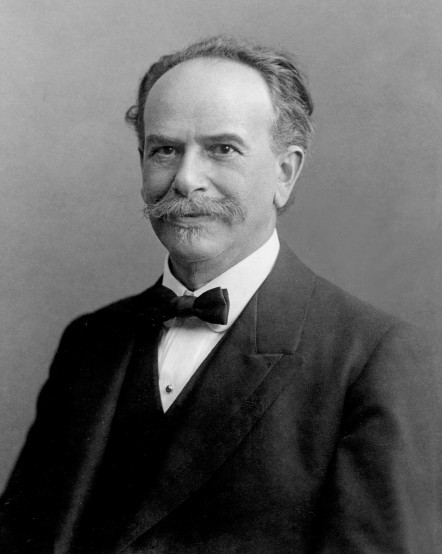
\includegraphics[width=.9\textwidth]{figures/FranzBoas.jpg}
  \caption{Franz Boas (1912)}
  \label{fig:ch.boas.boas}
\end{wrapfigure}
On the other hand, {\Boas}'s descriptions (and those influenced directly
by him) are thoroughly explicit in bringing out, through a system of
rules for the composition of forms (including both `\isi{phonotactics}' and
`\isi{euphonic laws}'), just what the limits are on the range of different
forms in the language. That these descriptions ``itemize'' in the sense
of recording as wide a range of forms as possible as accurately as
possible is of course true. We could only conclude that they do not
``structure'' the languages with which they deal, however, if we were to
accept the notion that the only way to elucidate the structure of a
language is in terms of an alternate representation of its forms,
which makes exactly the distinctive \isi{oppositions} explicit.

We conclude, therefore, that {\Boas}'s phonology falls rather
straightforwardly within the `\isi{fully specified surface variant}' view
sketched above in chapter~\ref{ch.saussure_sound}. That is, the only
significant representation of utterances is a surface-phonetic
form—but a complete grammar also contains, in addition to such
\isi{representations}, a system of rules which describe predictabilities of
various sorts in (a) the range of shapes of possible utterances, and
(b) the \isi{systematic relations} in shape that arise between distinct but
related utterances.

{\Boas}'s view of phonological form, then, is rather similar to that of
{\Saussure}. Of course, {\Boas} attributes much less theoretical importance
to the fact of distinctness of forms than did {\Saussure}, but the rules
of a grammar constructed according to his views nonetheless express
quite rigorously those variations in shape that are possible within
the `same' linguistic element, as opposed to those which must
correspond to an opposition between different elements. {\Saussure}'s
interest was largely theoretical, and it is thus necessary to infer
most of the practical consequences of his views (as discussed in
chapters~\ref{ch.saussure_life} and~\ref{ch.saussure_sound} above),
while the situation is almost exactly reversed in {\Boas}'s
case. Nonetheless, if the interpretations I have given here are
correct, the actual substance of the conception of phonological
structure held by the pioneers of European and of American linguistics
in the twentieth century was strikingly similar.

%%% Local Variables: 
%%% mode: latex
%%% TeX-master: "/Users/sra/Dropbox/Docs/Books/P20C_2/LSP/main.tex"
%%% End: 

